% LTeX: language=pl-PL
\documentclass[a4paper, 11pt, twoside, final]{memoir}

\usepackage{graphicx}
\usepackage{polski}
\usepackage[utf8]{inputenc}
\usepackage{amsmath}
\usepackage{amssymb}
\usepackage{physics}
\usepackage{bbold}
\usepackage[makeindex]{imakeidx}
\usepackage{qcircuit}
\usepackage{pdfpages}
\usepackage{pgffor}
\usepackage{colortbl}
\usepackage{tikz}
\usepackage{indentfirst}
\usepackage{xcolor}
\usepackage{soulutf8}
\usepackage{listings}
\usepackage{float}
\usepackage{longtable}
\usepackage{epigraph}
\usepackage{ragged2e}
\usepackage[hidelinks]{hyperref}
\usepackage[inline]{enumitem}

\usetikzlibrary{backgrounds,fit,decorations.pathreplacing,quotes,angles}

\makeindex[options=-s lou3.ist]
\indexsetup{level=\chapter*,firstpagestyle=chapter}

\newsubfloat{figure}

\renewcommand{\i}{{\mathrm i}}
\newcommand{\id}{I}
\newcommand{\Complex}{\mathbb{C}}
\newcommand{\Real}{\mathbb{R}}
\newcommand{\Field}{\mathbb{F}}
\newcommand{\conj}[1]{{#1}^*}
\newcommand{\mat}[1]{\mathbf{#1}}
\newcommand{\newterm}[1]{\emph{#1}}
\makeatletter
\newcommand{\chapterauthor}[1]{%
	{\parindent0pt\vspace*{-25pt}%
		\linespread{1.1}\large\scshape#1%
		\par\nobreak\vspace*{35pt}}
	\@afterheading%
}
\makeatother

\title{}
\author{}
\begin{document}

% LTeX: language=pl-PL
\chapter{Mechanika kwantowa}
\chapterauthor{PG}
% +Oskar Słowik w wydaniu 2

Mechanika kwantowa opisuje zachowania bardzo małych cząstek fizycznych,
czyli~np.~fotonów, elektronów albo~kwantowych bitów -- kubitów.
Na~potrzeby niniejszej~książki przyjmiemy, że~nie~będą nas interesować
ich właściwości fizyczne, a~tylko pewne abstrakcyjne stany,
w~jakich~mogą~się znajdować. Stany te numerujemy zazwyczaj przy~użyciu
liczb naturalnych: 0, 1, 2 itd. Stany kwantowe opisują np. polaryzację
fotonu, energię elektronu na~orbicie atomu, drgania sieci krystalicznej,
spin cząstki lub~jeszcze~inne właściwości układów kwantowych.

Informatyków często nie~interesuje, w~jaki~sposób właściwości fizyczne układów
są~wykorzystywane do~zapisu informacji klasycznej w~komputerze klasycznym --
a~zauważmy, że~do~tego~celu może zostać wykorzystana magnetyzacja powierzchni na
talerzu dysku twardego, napięcie elektryczne w~obwodzie wewnątrz procesora czy~wartość
natężenia prądu w~przewodzie elektrycznym. Dlatego też informatyków kwantowych nie~musi
interesować to, w~jaki sposób informacja kwantowa jest fizycznie zapisana
w~komputerze kwantowym.

Gdy~mówimy o~mechanice kwantowej, a~zatem również~o~informatyce kwantowej, posługujemy~się
fizycznym pojęciem \emph{doświadczenia}. Doświadczenie -- w~znaczeniu, jakie~będziemy
nadawać mu w~niniejszym tekście -- składa~się z~trzech etapów:
\begin{itemize}
	\item przygotowania,
	\item ewolucji,
	\item pomiaru i~interpretacji wyników.
\end{itemize}

W~interesującym nas~kontekście możemy opisać poszczególne etapy doświadczenia
następująco: przygotowujemy stan kwantowy, przeprowadzamy ewolucję kwantową
tego~stanu i -- na~koniec -- wykonujemy pomiar kwantowy (patrz:
Rysunek~\ref{rys:doswiadczenie}).
\begin{figure}[t]
	\centering
	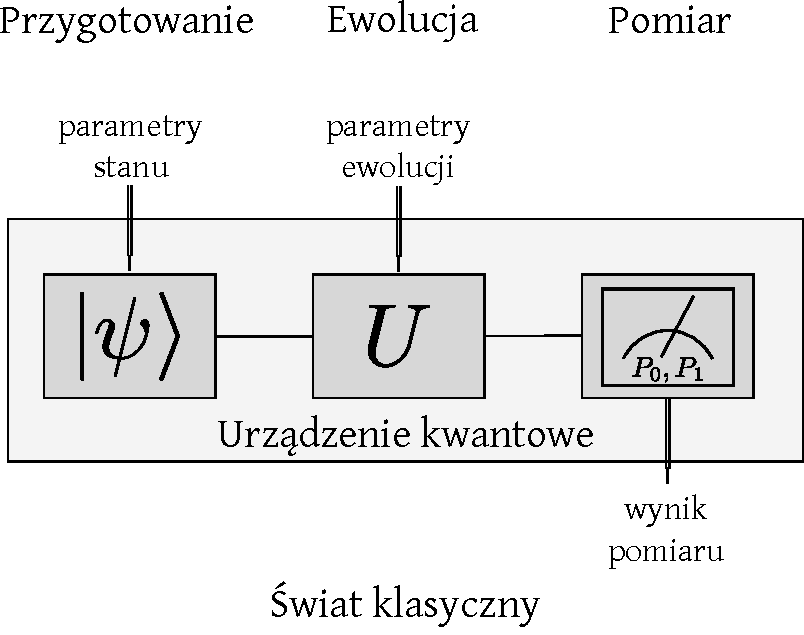
\includegraphics[width=0.7\textwidth]{pics/eksperymentkwantowy}
	\caption{Schematyczna reprezentacja doświadczenia kwantowego}
	\label{rys:doswiadczenie}
\end{figure}

Zauważmy, że~w~podobny sposób wykonujemy w~informatyce obliczenia klasyczne:
przygotowujemy dane (stan początkowy); następnie wykonujemy program (ewolucja)
i~odczytujemy wynik (pomiar). Współczesne komputery wykonują te~trzy etapy jako~przeprowadzane
nieustannie obliczenia. Nie~obserwujemy tych etapów podczas~codziennych
interakcji z~komputerem, więc nie~zauważamy w~sposób świadomy powyższego schematu
działania.

Każde urządzenie informatyczne działające na~podstawie zasad informatyki
kwantowej -- lub,~w~skrócie,
komputer kwantowy -- musi być wyposażone zarówno w~podukład kwantowy,
jak~i~podukład klasyczny, czyli~jakąś~formę komputera klasycznego,
np.~elektronicznego.
Komputer klasyczny będzie w~takim urządzeniu odpowiadał za~sterowanie układem
kwantowym, komunikację ze~światem zewnętrznym oraz~interpretację wyników
działania komputera kwantowego. Schemat konstrukcji i~działania komputera
kwantowego sprzężonego z~komputerem klasycznym
przedstawiono na~Rysunku~\ref{rys:komputer}.
\begin{figure}
	\centering
	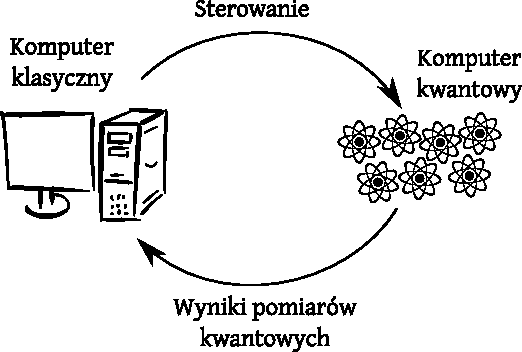
\includegraphics[width=0.7\textwidth]{pics/sterowaniepomiar}
	\caption{Schematyczna reprezentacja działania kwantowego urządzenia informatycznego. Komputer klasyczny steruje
		komputerem kwantowym, komputer kwantowy zwraca wyniki pomiarów do komputera klasycznego.}
	\label{rys:komputer}
	% https://openclipart.org/detail/15831/stylized-atom
	% https://openclipart.org/detail/1953/minimalist-monitor-and-computer
\end{figure}

W~przypadku bardziej~złożonym -- kiedy~chcemy opisać sieć komputerów kwantowych
i~jej wykorzystanie -- mówimy zazwyczaj również~o~użytkownikach tej sieci, którzy
mają do~dyspozycji komputery kwantowe i~klasyczne oraz~kwantowe i~klasyczne
połączenia sieciowe. Na~potrzeby opisu w~literaturze przedmiotu nadaje im~się umowne imiona:
,,Alicja'' (użytkownik A), ,,Bob'' (użytkownik B) oraz~,,Ewa'' (podsłuchujący)%
\footnote{Po~angielsku -- ,,Alice'', ,,Bob'' i~,,Eve''. Imiona ,,Alice'' i~,,Bob'' są używane, ponieważ~można
	je oznaczyć literami A i~B, natomiast~,,Eve'' pochodzi od~angielskiego słowa \emph{eavesdropping} -- czyli~podsłuchiwanie.}.
Pierwsze dwie osoby próbują się~komunikować, a~ostatnia próbuje im w~tym przeszkodzić.
Nietrudno zauważyć, że~w~komiksie dość~swobodnie nawiązujemy do~tej konwencji.

\section{Formalizm matematyczny}
Mechanika kwantowa jest opisywana przy~pomocy formalizmu (czyli języka)
matematycznego, który wykorzystuje liczby zespolone, wektory oraz~macierze.
Bez~jego zrozumienia nie~jest zatem możliwe zrozumienie samej mechaniki
kwantowej. Jednakże~w~niniejszej książce najpierw skupimy~się na~przedstawieniu
pojęć ściśle związanych z~mechaniką i~informatyką kwantową, natomiast~opis
formalizmu matematycznego znajdziesz w~rozdziale~\ref{ch:podstawy} zamieszczonym na~końcu.
Uznaliśmy~bowiem, że~nie~chcemy Cię zmuszać do~nauki materiału
matematycznego, skoro jeszcze nie~znasz powodów, dla~których opanowanie tego
formalizmu jest Ci~niezbędne. Oczywiście możesz zacząć od~lektury rozdziału~\ref{ch:podstawy} --
a~jeśli~się~na~nią nie~zdecydujesz, zachęcamy do~zerkania do~niego, ilekroć
nie~będziesz rozumieć jakiegoś pojęcia lub~symbolu matematycznego.

\section{Kubit}
Elementarnym obiektem w~informatyce kwantowej jest \newterm{kubit}\index{kubit},
który jest najprostszym układem kwantowym. Stan kubitu (zdefiniowany poniżej) opisuje wektor o~dwóch
elementach zespolonych.

W~celu opisania stanu kubitu zwyczajowo wybieramy bazę obliczeniową
$$
	\ket{0}=\begin{bmatrix} 1\\ 0\end{bmatrix},
	\ket{1}=\begin{bmatrix} 0\\ 1\end{bmatrix}.
$$
Wówczas dowolny stan $\ket{\psi}$ kubitu tworzy liniową kombinację wektorów bazowych
$$
	\ket{\psi}=\alpha\ket{0}+\beta\ket{1},
	\label{equ:kubit}
$$ z~$|\alpha|^2+|\beta|^2=1$ oraz $\alpha, \beta \in
	\Complex$.

Liczby $\alpha$ i~$\beta$ są zespolone, zatem aby~je zapisać, potrzebujemy
czterech liczb rzeczywistych. Jednak~ponieważ zachodzi warunek $|\alpha|^2+|\beta|^2=1$,
jedną z~potrzebnych nam liczb możemy wyliczyć z~pozostałych trzech. Wynika z~tego,
że~dowolny stan kubitu może być opisany przez~trzy liczby rzeczywiste.
Taki przykładowy opis jest zadany równaniem
$$
	\ket{\psi}=e^{\i\gamma}\left(
	\cos{\frac{\theta}{2}}\ket{0}+e^{\i\phi}\sin{\frac{\theta}{2}}\ket{1}
	\right),
$$
gdzie~$\gamma, \theta, \phi\in\mathbb{R}$.
Współczynnik $e^{\i\gamma}$ nazywamy \newterm{fazą globalną}\index{faza
	globalna}. Jak~się~później przekonamy, nie~ma on większego znaczenia, więc~zawsze
możemy przyjmować, że~równa~się on 1, czyli~$\gamma=0$. Zatem w~efekcie
dostajemy taką~oto~postać wzoru stanu kubitu:
$$
	\ket{\psi}=
	\cos{\frac{\theta}{2}}\ket{0}+e^{\i\phi}\sin{\frac{\theta}{2}}\ket{1}.
$$

Jeżeli dwa stany różnią~się fazą globalną, to fizycznie te stany są takie
same. Zatem każdy stan możemy również pomnożyć przez~dowolną liczbę w~postaci
$e^{\i\gamma}$, nie~zmieniając tego stanu.

Liczby rzeczywiste $\theta$ i~$\phi$ mogą być interpretowane jako~współrzędne
punktu na~trójwymiarowej sferze o~promieniu 1. Sferę taką~nazywamy
\emph{sferą Blocha}\index{sfera Blocha}. Będziemy ją bardzo często wykorzystywać
do~wizualizacji operacji na~kubicie.

\subsection{Sfera Blocha}
\begin{figure}[h]
	\begin{center}
		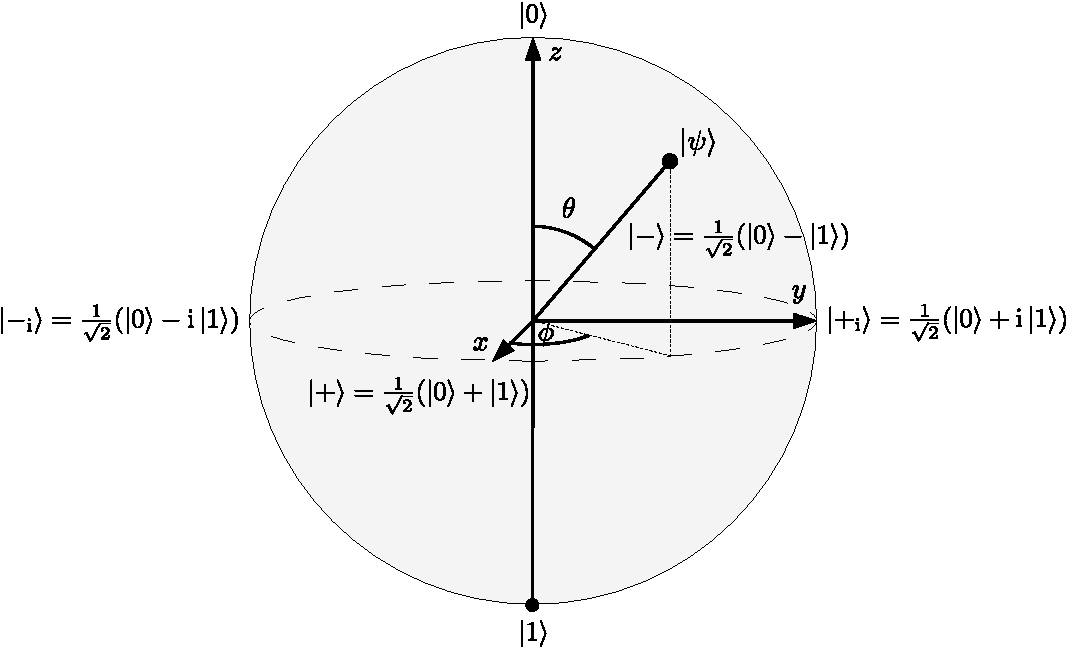
\includegraphics[width=0.8\textwidth]{pics/bloch}
	\end{center}
	\caption{Sfera Blocha}
	\label{rys:sferablocha}
\end{figure}
Sfera Blocha\footnote{Od nazwiska szwajcarskiego fizyka Feliksa Blocha
	(1905 -- 1983).} (Rysunek~\ref{rys:sferablocha}) jest wygodną
reprezentacją graficzną kubitu. Na powierzchni sfery Blocha znajdują się
punkty odpowiadające stanom kwantowym. Zazwyczaj rysujemy ją
w~taki~sposób, że~stan $\ket{0}$ oznaczamy u~góry, stan $\ket{1}$
u~dołu,
$\ket{-_\i}=\frac{1}{\sqrt{2}} (\ket{0}-\i\ket{1})$ po~lewej stronie,
$\ket{+_\i}=\frac{1}{\sqrt{2}}
	(\ket{0}+\i\ket{1})$ -- po~prawej, $\ket{+}=\frac{1}{\sqrt{2}} (\ket{0}+\ket{1})$ z~przodu,
a~$\ket{-}=\frac{1}{\sqrt{2}} (\ket{0}-\ket{1})$ z~tyłu.

W~dalszej części tekstu zostanie opisane, w~jaki~sposób bramki kwantowe działają
na~kubit -- a~odwzorowania zostaną zaprezentowane właśnie na~sferze Blocha.

\section{Stan}
\emph{Stanem}\index{stan!kwantowy} w~mechanice kwantowej nazywamy wektor
$$
	\ket{\psi}=
	\begin{bmatrix}
		\alpha_0 \\
		\alpha_1 \\
		\vdots   \\
		\alpha_{n-1}
	\end{bmatrix},
$$
który możemy zapisać również w~bazie obliczeniowej w~postaci
$$
	\ket{\psi}=\alpha_0\ket{0} + \alpha_1 \ket{1} + \ldots + \alpha_{n-1} \ket{n-1}.
$$
Chcemy, aby~$\alpha_i \in \Complex$ dla~$i=0, 1, \ldots, n-1$, tzn.~współczynniki
wektora, były liczbami zespolonymi, oraz~aby~$\norm{\ket{\psi}} = \sqrt{\abs{\alpha_0}^2
		+ \abs{\alpha_1}^2 + \ldots + \abs{\alpha_{n-1}}^2} = 1$, tzn.~aby~norma
euklidesowa wektora\index{wektor!norma euklidesowa} wynosiła
1\footnote{Zauważ, że baza obliczeniowa jest ortonormalna\index{baza
		ortonormalna}.}.

Liczby $\alpha_i \in \Complex$ nazywamy
\emph{amplitudami prawdopodobieństwa}\index{amplituda prawdopodobieństwa} stanu kwantowego. Gdy~jedna
z~tych liczb jest równa 1, możemy powiedzieć -- nieformalnie -- że~układ
kwantowy jest w~stanie odpowiadającym tej liczbie. Na~przykład jeżeli~$\alpha_0=1$,
mówimy, że~układ kwantowy jest w~stanie $\ket{0}$.

Jeżeli żadna z~liczb $\alpha_i$ nie~jest równa 1, to~znaczy, że~przynajmniej dwie
amplitudy prawdopodobieństwa są niezerowe. Wówczas mówimy, że~układ jest w~\emph{superpozycji}
stanów\index{superpozycja}. Przykładowo: jeżeli mamy układ z~$n=3$ i~$\alpha_0 = \alpha_2 = 1/\sqrt{2}$, tzn.~nasz
stan zapisujemy jako~$1/\sqrt{2}\ket{0}+1/\sqrt{2}\ket{2}$, to~mówimy, że~stan
jest w~superpozycji stanu $\ket{0}$ oraz~$\ket{2}$.

\section{Stany wielosystemowe}
\subsection{Dwa kubity}
Operacją matematyczną, która~odpowiada złączeniu układów dwóch kubitów, jest
\newterm{iloczyn Kroneckera}\footnote{Od nazwiska niemieckiego matematyka Leopolda Kroneckera (1823 -- 1891).}\index{iloczyn Kroneckera}.
Jeśli dane są stany dwóch kubitów $\ket{\psi}$ i~$\ket{\phi}$:
$$
	\ket{\psi}=
	\begin{bmatrix}
		\alpha \\
		\beta
	\end{bmatrix}
	=\alpha\ket{0}+\beta\ket{1}
	,
	\ket{\phi}=
	\begin{bmatrix}
		\gamma \\
		\delta
	\end{bmatrix}
	= \gamma\ket{0}+ \delta\ket{1},
$$
to ich~łączny stan zapisujemy następująco:
$$
	\ket{\psi}\otimes\ket{\phi}=
	\begin{bmatrix}
		\alpha \gamma \\
		\alpha \delta \\
		\beta \gamma  \\
		\beta \delta
	\end{bmatrix}=
	\alpha \gamma\ket{0}\otimes\ket{0}+
	\alpha \delta\ket{0}\otimes\ket{1}+
	\beta \gamma\ket{1}\otimes\ket{0}+
	\beta \delta\ket{1}\otimes\ket{1},
$$
bądź~w~skrócie:
$$
	\ket{\psi\phi}=
	\alpha \gamma\ket{00}+
	\alpha \delta\ket{01}+
	\beta \gamma\ket{10}+
	\beta \delta\ket{11}.
$$

Jak~widać, etykiety $00$, $01$, $10$ oraz~$11$ odpowiadają liczbom $0$, $1$, $2$
oraz~$3$ zapisanym binarnie.
Zatem stan $\ket{\psi\phi}$ możemy zapisać jako:
$$
	\ket{\psi\phi} =
	\alpha \gamma\ket{0}+
	\alpha \delta\ket{1}+
	\beta \gamma\ket{2}+
	\beta \delta\ket{3}.
$$
Zapiszmy teraz nowy stan:
$$
	\ket{\Phi} = c_0\ket{0} + c_1\ket{1} + c_2\ket{2} + c_3\ket{3}
$$
i~zastanówmy się, czy~istnieją takie~liczby $c_0, c_1, c_2, c_3$,
dla~których nie~da~się znaleźć takich~$\alpha, \beta, \gamma, \delta$,
które spełniają układ równań $$c_0=\alpha \gamma,\; c_1=\alpha \delta,\; c_2=\beta \gamma,
	\text{ oraz } c_3=\beta \delta.$$

Weźmy pod~uwagę stan $\ket{\Phi^+}=\frac{1}{\sqrt{2}}(\ket{0}+\ket{3})$
i~dla~uproszczenia opuśćmy czynnik $\frac{1}{\sqrt{2}}$. Wtedy~mamy
$c_0=c_3=1$ oraz~$c_1=c_2=0$. Załóżmy, że~nasz stan możemy zapisać w~postaci
$\alpha \gamma\ket{0}+ \alpha \delta\ket{1}+\beta
	\gamma\ket{2}+\beta \delta\ket{3}$. Wówczas uzyskujemy układ równań:
$$\alpha \gamma=1,\; \alpha \delta=0,\; \beta\gamma=0,\; \beta\delta=1.$$
Zauważmy, że~$\alpha,
	\beta, \gamma, \delta \geq 0$, co~wynika z~tego, że~$|\alpha|^2+|\beta|^2 = 1$
oraz~$|\delta|^2+|\gamma|^2 = 1$. Zatem aby~spełnić pierwszy warunek $\alpha = \gamma = 1$,
natomiast aby~spełnić drugi warunek $\delta = 0$.
Jednakże~z~czwartego warunku wynika, że~$\delta = 1$. Zatem otrzymujemy
sprzeczność. Wnioskujemy z~tego, że~stanu $\ket{\Phi^+}$ nie~da~się zapisać jako iloczynu
Kroneckera dwóch stanów. Stan $\ket{\Phi^+}$ nazywamy \newterm{stanem
	Bella}\index{stan!Bella}\footnote{Od~nazwiska brytyjskiego fizyka Johna S.~Bella (1928 -- 1990).}. Ma on
wyjątkowo istotne znaczenie w~informatyce kwantowej.

\subsection{Wiele układów kwantowych}
Gdy~mamy do~dyspozycji $n$ kubitów w~stanach
$$\ket{\psi_1}, \ket{\psi_2}, \ldots, \ket{\psi_n},$$
wówczas~możemy opisać je jako~jeden łączny układ, którego~stan ma
$2^n$ współczynników. Operacją matematyczną,
która w~sposób zbiorczy opisuje takie~połączenie wielu kubitów, jest
iloczyn Kroneckera. Jeżeli~kubity nie~są ze~sobą związane (splątane), to stan
takiego układu jest opisany przez~łączny stan
$$
	\ket{\Psi}=\ket{\psi_1}\otimes \ket{\psi_2}\otimes \ldots\otimes \ket{\psi_n}.
$$

\subsection{Splątanie kwantowe}
Splątanie kwantowe jest zjawiskiem, które dotyczy tylko~i~wyłącznie obiektów
podlegających prawom mechaniki kwantowej. Splątane mogą być dwa układy (lub~więcej), które miały okazję ze~sobą
oddziaływać w~przeszłości. Matematycznie definicja
splątania dwóch układów jest następująca: jeżeli~danego stanu $\ket{\phi}$,
który opisuje stan dwóch układów, nie~możemy
zapisać jako~$\ket{\psi_1}\otimes\ket{\psi_2}$ dla~jakichkolwiek $\ket{\psi_1}$
oraz~$\ket{\psi_2}$, to jest on \newterm{splątany}\index{stan!splątany}. Jeżeli~natomiast
istnieją takie $\ket{\psi_1}$ oraz~$\ket{\psi_2}$, że~$\ket{\phi}=\ket{\psi_1} \otimes \ket{\psi_2}$, to stan nazywamy
\newterm{separowalnym}\index{stan!separowalny}.
Jak widać, wspomniany wcześniej stan Bella $\ket{\Phi^+}$ jest stanem
splątanym.

Splątanie wielu układów kwantowych\index{stan!splątany!wiele układów kwantowych} jest problemem znacznie bardziej~złożonym. Jeżeli~mamy
np.~trzy układy, to pierwsze dwa mogą być splątane ze~sobą, ale~nie~z~trzecim,
jak~na~przykład w~stanie
$$
	\frac{1}{\sqrt{2}}(\ket{00}+\ket{11})\otimes \ket{1}.
$$
Wszystkie trzy układy mogą być ze~sobą splątane na~różne sposoby. Przykładowo stany
$$
	\ket{W}=\frac{1}{\sqrt{3}}(\ket{001}+\ket{010}+\ket{100})
$$
oraz
$$
	\ket{GHZ}=\frac{1}{\sqrt{2}}(\ket{000}+\ket{111})
$$
są splątane w~całkowicie różny sposób -- przy~czym~wytłumaczenie tego faktu wykracza poza~zakres tej książki.

Stany splątane mają bardzo nieintuicyjne właściwości. Na przykład,
jeżeli cząstki będące w~stanie splątanym oddalimy bardzo daleko
od~siebie, pozostaną one ze~sobą związane. Będziemy mieli okazję
zaobserwować ten efekt, gdy~będzie mowa o~pomiarze stanów splątanych.

\section{Ewolucja kwantowa}
\newterm{Ewolucja kwantowa}\index{ewolucja kwantowa}
to nazwa, którą opisujemy zmianę stanu kwantowego w~czasie. Zakładamy, że~mamy
pewien stan w~chwili $0$, a~dzięki ewolucji kwantowej uzyskujemy stan w~chwili $1$.
Zwróćmy tutaj uwagę na~pewien fakt dotyczący stanów kwantowych: norma stanu kwantowego wynosi zawsze 1.
Normę tę utożsamiamy z~prawdopodobieństwem całkowitym. Zatem jeżeli~chcemy, by~prawdopodobieństwo
całkowite było zachowane, oznacza to, że~chcemy, by matematyczny opis
ewolucji zachowywał normę wektora stanu. Norma wektora jest zachowywana
wyłącznie przez~obroty i~symetrie. Taki opis matematyczny ewolucji możemy uzyskać z wykorzystaniem macierzy
unitarnych. Dla~uproszczenia opisu pomijamy tutaj kwestię wymiarów macierzy
i~wektorów stanów. Oczywiście wymiary muszą być tak dobrane, by można było
mnożyć odpowiadające sobie~nawzajem wymiarami macierze i~wektory.

Przejście ze~stanu w~chwili $0$ $\ket{\psi_{t=0}}$ do~stanu w~chwili
$1$ $\ket{\psi_{t=1}}$ jest zadane przez
$
	\ket{\psi_{t=1}}= \mat{U}\ket{\psi_{t=0}},
$
gdzie~$\mat{U}$ jest macierzą unitarną.

Powyższe, pozornie trywialne, równanie opisuje zachowanie wszystkich układów kwantowomechanicznych, w~tym oczywiście
komputerów kwantowych. W~informatyce kwantowej macierze unitarne\index{macierz!unitarna} przeważnie
nazywamy \newterm{bramkami kwantowymi}\index{bramka!kwantowa}.

Zauważmy od~razu pewną charakterystyczną cechę mechaniki kwantowej, wynikającą z~powyższego
równania: pamiętając, że~macierz odwrotna $\mat{U}^{-1}$ do~macierzy
unitarnej zawsze istnieje i~jest jej sprzężeniem hermitowskim $\mat{U}^\dagger$,
możemy zapisać to równanie odwrócone w~czasie:
$
	\ket{\psi_{t=0}}= \mat{U}^\dagger\ket{\psi_{t=1}}.
$
Dlatego~też~mówimy, że~ewolucja kwantowa jest \emph{odwracalna w~czasie}.

\section{Bramki kwantowe}
Bramek kwantowych jest nieskończenie wiele -- jednakże~my, mimo~ich mnogości,
skupimy~się tylko na~bramkach działających na~jeden lub~dwa kubity. Bramki te
wystarczają do~tego, by zbudować dowolny komputer kwantowy lub~kwantowe
urządzenie komunikacyjne. Są one zatem najciekawsze z~punktu widzenia
informatyka kwantowego.

\subsection{Bramki jednokubitowe}
Dla~jednego kubitu możemy zapisać wiele różnych bramek kwantowych\index{bramka!jednokubitowa}.
Na~początek zdefiniujmy bramkę obrotu wokół osi~$y$ o~kąt~$\gamma$:
$$
	\mat{R_y}(\gamma)=
	\begin{bmatrix}
		\cos({\frac{\gamma}{2}})  & \sin({\frac{\gamma}{2}}) \\
		-\sin({\frac{\gamma}{2}}) & \cos({\frac{\gamma}{2}})
	\end{bmatrix},
$$
bramkę obrotu wokół osi~$z$ o~kąt~$\beta$:
$$
	\mat{R_z}(\beta)=
	\begin{bmatrix}
		e^{\frac{\i\beta}{2}} & 0                      \\
		0                     & e^{\frac{-\i\beta}{2}}
	\end{bmatrix}
$$
oraz~bramkę zmieniającą fazę globalną o~czynnik~$\alpha$:
$$
	\mat{Ph(\alpha)}=
	\begin{bmatrix}
		e^{\i\alpha} & 0            \\
		0            & e^{\i\alpha}
	\end{bmatrix}.
$$
Działanie bramek $\mat{R_z}(\beta)$ oraz~$\mat{R_y}(\gamma)$ zostało pokazane na~Rysunku \ref{rys:bramki-obrotów}.
Bramka $\mat{Ph(\alpha)}$ zmienia tylko globalną fazę, zatem jej działania nie~można zaobserwować na~sferze Blocha.

Dowolna bramka działająca na~jednym kubicie może zostać zapisana jako złożenie
czterech bramek: zmiany fazy oraz trzech obrotów, w~postaci
opisanej przez~cztery liczby rzeczywiste $\alpha, \beta, \gamma, \delta$:
\begin{equation*}
	\begin{split}
		\mat{U}(\alpha, \beta, \gamma, \delta)=&
		\mat{Ph}(\alpha)\mat{R_z}(\beta)\mat{R_y}(\gamma)\mat{R_z}(\delta)
		=\\
		=&
		\begin{bmatrix}
			e^{\i\alpha} & 0            \\
			0            & e^{\i\alpha}
		\end{bmatrix}
		\begin{bmatrix}
			e^{\frac{\i\beta}{2}} & 0                      \\
			0                     & e^{\frac{-\i\beta}{2}}
		\end{bmatrix}
		\begin{bmatrix}
			\cos({\frac{\gamma}{2}})  & \sin({\frac{\gamma}{2}}) \\
			-\sin({\frac{\gamma}{2}}) & \cos({\frac{\gamma}{2}})
		\end{bmatrix}
		\begin{bmatrix}
			e^{\frac{\i\delta}{2}} & 0                       \\
			0                      & e^{\frac{-\i\delta}{2}}
		\end{bmatrix}
		.
	\end{split}
\end{equation*}
Pierwszy obrót to obrót wokół osi~$z$, drugi -- wokół osi~$y$, a~trzeci -- ponownie wokół $z$.

\begin{figure}
	\centering
	\subbottom[Bramka $\mat{R_z}(\beta)$ dokonująca obrotu wokół osi $z$ łączącej $\ket{0}$ z~$\ket{1}$.
		\label{rys:bramka-rz}]{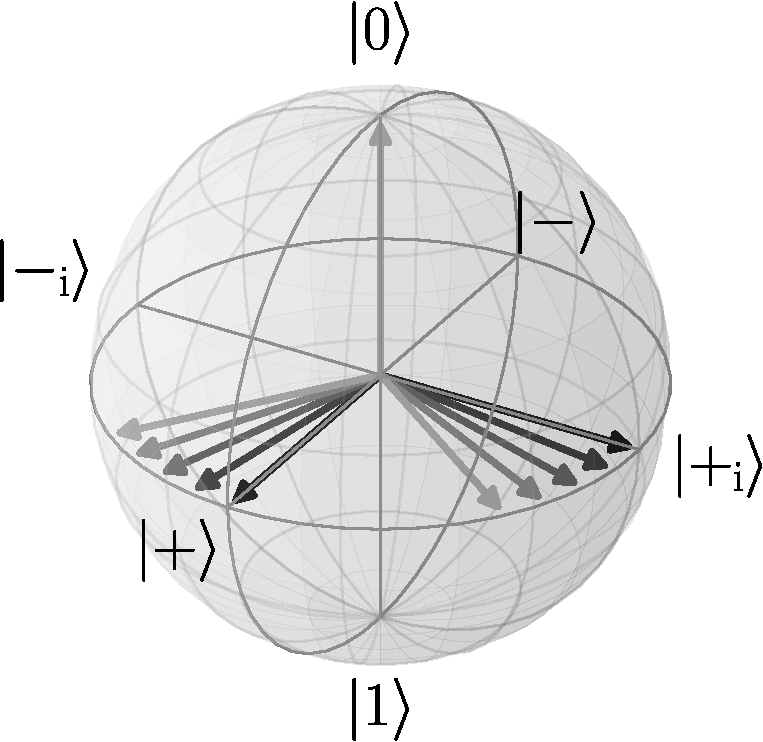
\includegraphics[width=0.46\linewidth]{pics/Rz}}
	\hfill
	\subbottom[Bramka $\mat{R_y}(\gamma)$ dokonująca obrotu wokół osi $y$ łączącej $\ket{+_\i}$
		z~$\ket{-_\i}$.\label{rys:bramka-ry}]{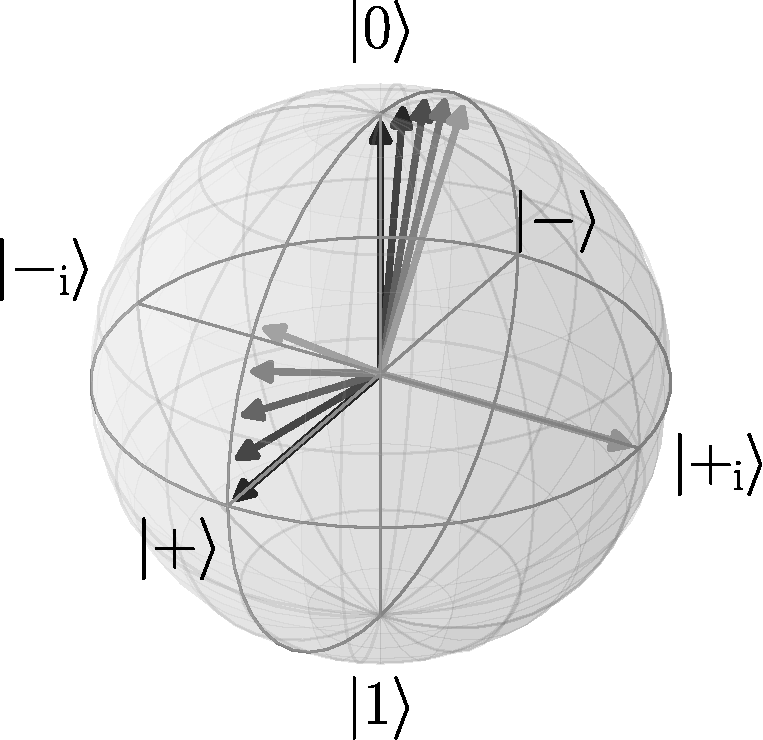
\includegraphics[width=0.46\linewidth]{pics/Ry}}
	\caption{Działanie bramek $\mat{R_z}(\beta)$ -- panel~\subcaptionref{rys:bramka-rz} oraz~$\mat{R_y}(\gamma)$
	-- panel~\subcaptionref{rys:bramka-ry} na~stanach $\ket{0}$, $\ket{+}$, $\ket{+_\i}$ (czarne strzałki).
	Wartości $\beta$ oraz~$\gamma$ rosną zgodnie z~przechodzeniem kolorów strzałek od~ciemniejszych
	do~jaśniejszych i~wynoszą $(0{,}05\pi,0{,}1\pi,0{,}15\pi,0{,}2\pi)$.
	}
	\label{rys:bramki-obrotów}
\end{figure}

Bramki kwantowe mają swoje oznaczenia graficzne. Bramkę
je\-dno\-ku\-bi\-to\-wą oznacza~się jako prostokąt, wewnątrz~którego zapisana jest nazwa
bramki. Przykład takiej bramki kwantowej pokazano na~Rysunku~\ref{rys:bramkakubitowa}.
\begin{figure}[h]
	\begin{center}
		\begin{minipage}{4in}
			\centering
			\Qcircuit @C=1em @R=.7em {
			\lstick{\ket{\psi}} & \gate{\mat{U}}  &  \rstick{\mat{U}\ket{\psi}} \qw
			}
		\end{minipage}
	\end{center}
	\caption{Rysunek przedstawiający bramkę jednokubitową $\mat{U}$. Pojedyncza
		linia przechodząca przez~bramkę oznacza kubit. Stan wejściowy do~bramki --
		po~lewej stronie, wyjściowy -- po~prawej.}
	\label{rys:bramkakubitowa}
\end{figure}

\subsubsection{Bramki jednokubitowe}
Kilka spośród~wszystkich bramek kwantowych\index{bramka!jednokubitowa} ma swoje ustalone nazwy, które są
często wykorzystywane w~informatyce kwantowej. Poniżej prezentujemy ich przegląd,
zawierający informację o~tym, jak~wygląda macierz danej bramki, jak działa ona
na~ogólny stan $\ket{\psi}=\alpha\ket{0} + \beta\ket{1}$, a~także
interpretację jej działania na~sferze Blocha.

\newterm{Bramka identyczność}\index{bramka!identyczność} nie~zmienia stanu kubitu.
Oznaczamy ją przez~$\mat{\id}$. Jej~macierz zawiera jedynki na~diagonali i~zera poza~diagonalą:
$$\mat{\id}=\begin{bmatrix} 1 & 0 \\ 0 & 1\end{bmatrix}.$$
Działanie identycznością na~stan jest trywialne:
$$\mat{\id}(\alpha\ket{0} + \beta\ket{1}) = \alpha\ket{0} + \beta\ket{1}.$$

\newterm{Bramka negacji bitu}\index{bramka!negacji bitu}
oznaczana jest przez~$\mat{X}$. Jej macierz jest następująca:
$$\mat{X}=\begin{bmatrix} 0 & 1 \\ 1 & 0\end{bmatrix},$$
a~działanie polega na~zamianie stanu $\ket{0}$ na~$\ket{1}$
i~odwrotnie. Zatem gdy~te stany bazy obliczeniowej są w~superpozycji,
bramka~$\mat{X}$ zamienia pomiędzy~nimi amplitudy prawdopodobieństwa:
$$\mat{X} (\alpha\ket{0} + \beta\ket{1}) = \alpha\ket{1} + \beta\ket{0}.$$

\newterm{Bramka negacji fazy}\index{bramka!negacji fazy}, oznaczana przez~$\mat{Y}$,
ma następującą postać macierzową:
$$\mat{Y} = \begin{bmatrix} 0&-\i\\ \i&0 \end{bmatrix}.$$
Jej działanie polega na~wzajemnej zamianie stanów $\ket{+}$ oraz~$\ket{-}$.
Jej działanie na~superpozycję stanów bazy obliczeniowej jest następujące:
$$\mat{Y} (\alpha\ket{0} + \beta\ket{1}) = \alpha\i\ket{1} - \beta\i \ket{0},$$
ale~ponieważ możemy pomnożyć ten stan przez~fazę globalną $\i=e^{\frac{\i \pi}{2}}$, nie~zmieniając
stanu, to otrzymujemy $\beta\ket{0}-\alpha\ket{1}$.

\newterm{Bramka negacji fazy i~bitu}\index{bramka!negacji fazy i~bitu} oznaczana jest przez~$\mat{Z}$,
a~jej macierz jest następująca:
$$\mat{Z} = \begin{bmatrix} 1 & 0 \\ 0 & -1\end{bmatrix}.$$
Bramka ta zamienia ze~sobą stany $\ket{+_\i}$ oraz~$\ket{-_\i}$.
Jej działanie na~superpozycji wektorów bazy obliczeniowej jest następujące:
$$\mat{Z} (\alpha\ket{0} + \beta\ket{1}) = \alpha\ket{0} - \beta\ket{1}.$$
Zauważmy, że~bramki $\mat{X}$, $\mat{Y}$ oraz~$\mat{Z}$ mają ciekawą własność:
$$\mat{X}^2=\mat{Y}^2=\mat{Z}^2=\i\mat{X}\mat{Y}\mat{Z}=\mat{\id}.$$

\newterm{Bramki zmiany fazy}\index{bramka!zmiany fazy}
to rodzina bramek $\mat{R}(\phi)$ zależnych od~parametru rzeczywistego $\phi$.
Postać macierzowa tych bramek jest następująca:
$$\mat{R}(\phi) = \begin{bmatrix} 1 & 0 \\ 0 & e^{\i \phi} \end{bmatrix}.$$
Ich działanie zmienia fazę względną pomiędzy~stanami bazy obliczeniowej:
$$\mat{R}(\phi) (\alpha\ket{0} + \beta\ket{1}) = \alpha\ket{0} +  e^{\i \phi} \beta\ket{1}.$$
Działanie tej rodziny bramek przedstawia Rysunek~\ref{rys:bramka-Rphi}.

\begin{figure}[h]
	\centering
	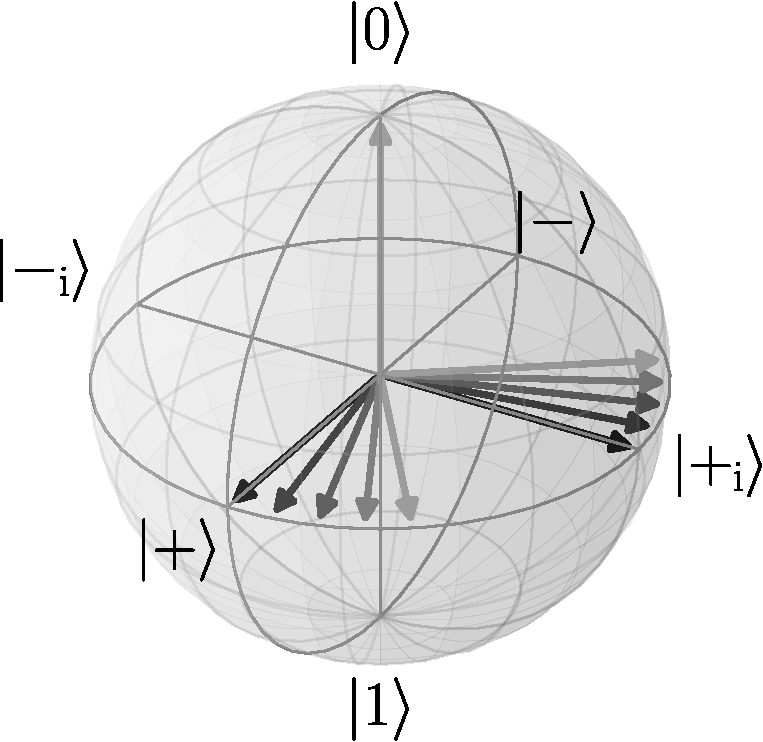
\includegraphics[width=0.45\linewidth]{pics/Rphi}
	\caption{Wizualizacja działania bramek $\mat{R}(\phi)$ na~stanach
	$\ket{0}$, $\ket{+}$, $\ket{+_\i}$ (czarne strzałki).
	Wartości $\phi$ rosną w~miarę rozjaśniania~się kolorów strzałek i~wynoszą
	$(0{,}05\pi,0{,}1\pi,0{,}15\pi,0{,}2\pi)$.}
	\label{rys:bramka-Rphi}
\end{figure}

\newterm{Bramka Hadamarda}\footnote{Od nazwiska francuskiego matematyka
	Jacquesa Salomona Hadamarda (1865 -- 1963).}\index{bramka!Hadamarda}
jest
oznaczana symbolem $\mat{H}$, a~jej postać macierzowa jest następująca:
$$\mat{H}=\frac{1}{\sqrt{2}} \begin{bmatrix} 1 & 1 \\ 1 & -1\end{bmatrix}.$$
Bramka ta jest często pierwszym krokiem wielu algorytmów i~protokołów
kwantowych, gdyż~przeprowadza ona stany bazy obliczeniowej
do~ich superpozycji\index{superpozycja} w~następujący sposób:
$$
	\begin{aligned}
		\mat{H}\ket{0} = \frac{1}{\sqrt{2}}\left( \ket{0} +\ket{1} \right)=\ket{+}, \\
		\mat{H}\ket{1} = \frac{1}{\sqrt{2}}\left( \ket{0} -\ket{1} \right)=\ket{-}.
	\end{aligned}
$$

Zauważmy, że bramka Hadamarda jest odwrotnością samej siebie, tzn. że $\mat{H} = \mat{H}^{-1}$. Zatem
$$
	\begin{aligned}
		\mat{H} \ket{+} = \ket{0}, \\
		\mat{H} \ket{-} = \ket{1}.
	\end{aligned}
$$

Wiedząc, że macierz bramki Hadamarda jest unitarna, tzn. że
$\mat{H}^{-1}=\mat{H}^\dagger$, widzimy, że $\mat{H}=\mat{H}^\dagger$. A
to oznacza, że macierz bramki Hadamarda jest macierzą
hermitowską\index{macierz!hermitowska}.

\subsection{Bramki kontrolowane} W~przypadku bramek dwukubitowych możemy
stworzyć bramki kontrolowane. O~bramkach tych mówimy, że~jeden kubit
kontroluje bramkę, a~na~drugi nakładana jest dana bramka
$\mat{U}$. Bramka kontrolowana\index{bramka kwantowa!kontrolowana} ,,kontrolowane~$\mat{U}$'' działa
w~następujący sposób: jeżeli~kubit kontrolujący\index{kubit!kontrolujący} jest w~stanie $\ket{1}$, to nałóż
wybraną bramkę $\mat{U}$ na~kubit docelowy\index{kubit!docelowy};
jeżeli~kubit kontrolujący jest w~stanie $\ket{0}$, to nie~rób nic.

Bramkę taką możemy zapisać w~postaci
$$
	\mat{C}\mat{U}_1^2=\ketbra{0}{0}\otimes \mat{\id} + \ketbra{1}{1}\otimes \mat{U},
$$
gdzie indeks dolny oznacza numer kubitu kontrolującego, a~górny kontrolowanego.
Jeżeli~bramka $\mat{U}$ ma postać macierzową
$$
	\mat{U}=
	\begin{bmatrix}
		u_{00} & u_{01} \\
		u_{10} & u_{11}
	\end{bmatrix},
$$
to kontrolowana bramka $\mat{U}$ ma postać
$$
	\mat{C}\mat{U}_1^2 = \begin{bmatrix} 1 & 0 & 0 & 0 \\ 0 & 1 & 0 & 0 \\ 0 & 0 & u_{00} & u_{01} \\ 0 & 0 & u_{10} & u_{11}  \end{bmatrix},
$$
a jej działanie można zapisać jako:
\begin{eqnarray}
	\mat{C}\mat{U}_1^2\ket{0}\otimes \ket{0} & = & \ket{0}\otimes \ket{0},\nonumber\\
	\mat{C}\mat{U}_1^2\ket{0}\otimes \ket{1} & = & \ket{0}\otimes \ket{0},\nonumber\\
	\mat{C}\mat{U}_1^2\ket{1}\otimes \ket{0} & = & \ket{1}\otimes \mat{U}\ket{0},\nonumber\\
	\mat{C}\mat{U}_1^2\ket{1}\otimes \ket{1} & = & \ket{1}\otimes \mat{U}\ket{1}.\nonumber
\end{eqnarray}
Na Rysunku~\ref{rys:bramkakontrolowana} pokazana jest graficzna reprezentacja
bramki ,,kontrolowane~$\mat{U}$''.
\begin{figure}[h]
	\begin{center}
		\begin{minipage}{2in}
			\Qcircuit @C=1em @R=.7em {
			& \ctrl{1}  & \qw \\
			& \gate{\mat{U}} & \qw
			}
		\end{minipage}
	\end{center}
	\caption{Rysunek przedstawiający bramkę kontrolowaną $\mat{U}$. Linie
		przechodzące przez~bramkę oznaczają kubity. Kropka oznacza kubit kontrolujący,
		a~kwadrat -- bramkę, która jest kontrolowana.}
	\label{rys:bramkakontrolowana}
\end{figure}

Natomiast jeżeli chcemy, by~w~bramce kontrolowanej kubit kontrolujący był drugi, a~kontrolowany
pierwszy, to możemy uzyskać taki efekt, korzystając z~następującej postaci bramki
$$\mat{C}\mat{U}_2^1=\mat{\id}\otimes\ketbra{0}{0} + \mat{U}\otimes\ketbra{1}{1}.$$

\subsubsection{Bramka $\mat{CNOT}$}
Bardzo użyteczną bramką kontrolowaną jest bramka
,,kontrolowane $\mat{X}$'', czyli~$\mat{CNOT}_1^2$\index{bramka!CNOT}\index{bramka!kontrolowane X}, która ma następującą postać
macierzową:
$$
	\mat{CNOT}_1^2 = \begin{bmatrix} 1 & 0 & 0 & 0 \\ 0 & 1 & 0 & 0 \\ 0 & 0 & 0 & 1 \\ 0 & 0 & 1 & 0  \end{bmatrix}.
$$

Działanie tej bramki można przedstawić następująco: jeżeli~kubit kontrolowany jest
w~stanie $\ket{0}$, to zaneguj stan kubitu docelowego. Zapis działania bramki będzie wyglądał wówczas tak:
\begin{eqnarray}
	\mat{CNOT}_1^2\ket{0}\otimes \ket{0} & = & \ket{0}\otimes \ket{0},\nonumber\\
	\mat{CNOT}_1^2\ket{0}\otimes \ket{1} & = & \ket{0}\otimes \ket{1},\nonumber\\
	\mat{CNOT}_1^2\ket{1}\otimes \ket{0} & = & \ket{1}\otimes \ket{1},\nonumber\\
	\mat{CNOT}_1^2\ket{1}\otimes \ket{1} & = & \ket{1}\otimes \ket{0}.\nonumber
\end{eqnarray}
Rysunek~\ref{rys:bramkaCNOT} pokazuje reprezentację graficzną tej bramki.
\begin{figure}[h]
	\begin{center}
		\begin{align*}
			\Qcircuit @C=1em @R=.7em {
			 & \ctrl{1} & \qw \\
			 & \targ    & \qw
			}
		\end{align*}
	\end{center}
	\caption{Rysunek przedstawiający bramkę $\mat{CNOT}_1^2$. Linia przechodząca przez~bramkę oznacza kubity.
		Kropka oznacza kubit kontrolujący, a~kółko z~krzyżykiem -- bramkę $\mat{X}$.}
	\label{rys:bramkaCNOT}
\end{figure}

\subsubsection{Bramka $\mat{SWAP}$}
Bramka $\mat{SWAP}$\index{bramka!SWAP} służy do~zamiany stanów dwóch kubitów. Można ją zrealizować
jako~ciąg trzech bramek: $\mat{CNOT}_1^2\mat{CNOT}_2^1\mat{CNOT}_1^2$, tak~jak~to przedstawiono
na~Rysunku~\ref{rys:bramkaswap}. Postać macierzowa bramki $\mat{SWAP}$ jest
następująca:
$$
	\mat{SWAP} = \begin{bmatrix} 1 & 0 & 0 & 0 \\ 0 & 0 & 1 & 0 \\ 0 & 1 & 0 & 0 \\ 0 & 0 & 0 & 1  \end{bmatrix}.
$$

\begin{figure}[h]
	\begin{center}
		\begin{minipage}{10em}
			\centering
			\begin{align*}
				\Qcircuit @C=1em @R=.7em {
				 & \ctrl{1} & \targ     & \ctrl{1} & \qw \\
				 & \targ    & \ctrl{-1} & \targ    & \qw
				}
			\end{align*}
		\end{minipage}
		\begin{minipage}{10em}
			\centering
			\begin{align*}
				\Qcircuit @C=1em @R=1.7em {
				 & \qswap \qw  & \qw \\
				 & \qswap \qwx & \qw
				}
			\end{align*}
		\end{minipage}
	\end{center}
	\caption{Rysunek po~lewej przedstawia ciąg bramek $\mat{CNOT}_1^2\mat{CNOT}_2^1\mat{CNOT}_1^2$,
		który~realizuje bramkę $\mat{SWAP}$ -- oznaczaną jak~na~rysunku po~prawej.}
	\label{rys:bramkaswap}
\end{figure}

\subsection{Łączenie bramek szeregowo}
Jeżeli~ewolucja kwantowa $\mat{U}$ jest podzielona w~czasie na~kolejne etapy,
tzn. na~przykład rozpoczyna~się od~bramki kwantowej $\mat{U}_{0\rightarrow 1}$,
która~przeprowadza stan z~chwili 0 do~chwili 1, a następnie wprowadza bramkę
kwantową $\mat{U}_{1\rightarrow 2}$, która~przeprowadza stan z~chwili 1
do~chwili 2 itd. \dots, aż~do~bramki
$\mat{U}_{(N-1)\rightarrow N}$, która~przeprowadza stan z~chwili $N-1$ do~chwili $N$ --
to taki~szereg ewolucji zapisujemy jako iloczyn macierzy
$$
	\mat{U} = \mat{U}_{(N-1)\rightarrow N}\mat{U}_{(N-2)\rightarrow (N-1)}\dots \mat{U}_{1\rightarrow 2} \mat{U}_{0\rightarrow 1}.
$$
W~takim~przypadku jako wynik otrzymujemy też~szereg stanów
$$\ket{\psi_1}=\mat{U}_{0\rightarrow 1}\ket{\psi_0},\;
	\ket{\psi_2}=\mat{U}_{1\rightarrow 2}\ket{\psi_1},\dots,\;
	\ket{\psi_N}=\mat{U}_{(N-1)\rightarrow N}\ket{\psi_{N-1}},$$
które odpowiadają kolejnym chwilom w~czasie.
Rysunek \ref{rys:bramkiszeregowo} przedstawia szeregowe łączenie bramek.
\begin{figure}[h]
	\begin{center}
		\begin{minipage}{4in}
			\centering
			\Qcircuit @C=1em @R=.7em {
			& \gate{\mat{U}_{0\rightarrow 1}} & \gate{\mat{U}_{1\rightarrow 2}} & \qw & \ldots  &  & \gate{\mat{U}_{{N-1}\rightarrow {N}}}  &   \qw
			}
		\end{minipage}
	\end{center}
	\caption{Szeregowe łączenie bramek kwantowych}
	\label{rys:bramkiszeregowo}
\end{figure}

\subsection{Łączenie bramek równolegle}
Jeżeli~mamy układ kwantowy składający~się z~wielu kubitów, to albo~każdy z~nich
może ewoluować oddzielnie,
albo~niektóre -- bądź~wszystkie -- mogą ewoluować łącznie.
Dodatkowo ewolucja niektórych (bądź~wszystkich) kubitów może być trywialna,
tzn.~niezmieniająca stanu.

Aby~można było połączyć bramki szeregowo, muszą one działać na~układ
składający~się z~takiej samej liczby kubitów. Nie~można łączyć bramek $\mat{X}$
i~$\mat{CNOT}_1^2$ szeregowo, gdyż~ich macierzy nie~można pomnożyć, ponieważ mają
różne wymiary. Zatem w~takim przypadku musimy rozszerzyć bramkę $\mat{X}$ tak,
by działała na~dwa kubity.
Wykorzystujemy do~tego iloczyn Kroneckera i~macierze identyczności.
Jeżeli~chcemy uzyskać ciąg bramek kwantowych taki,
w~którym na~początku działamy bramką $\mat{X}$ na~pierwszy kubit, a~następnie
bramką $\mat{CNOT}_1^2$ na~kubit pierwszy
(kontrolujący) i~kubit drugi (docelowy), to~rozszerzamy bramkę $\mat{X}$ tak, by
na~drugi kubit działała trywialnie do~postaci $\mat{X}\otimes \mat{\id}$. Pokazano to
na~Rysunku~\ref{rys:bramkirównolegle}.

\begin{figure}[h]
	\begin{center}
		\begin{minipage}{10em}
			\centering
			\begin{align*}
				\Qcircuit @C=1em @R=.7em {
				 & \gate{\mat{X}} & \ctrl{1} & \qw \\
				 & \qw            & \targ    & \qw
				}
			\end{align*}
		\end{minipage}
	\end{center}
	\caption{Graficzna reprezentacja operacji $\mat{CNOT}_1^2(\mat{X}\otimes \mat{\id})$}
	\label{rys:bramkirównolegle}
\end{figure}

\subsection{Obwody kwantowe}
Łączenie bramek szeregowo i~równolegle możemy przedstawić graficznie na~tzw.
\newterm{obwodzie kwantowym}\index{obwód kwantowy} -- czyli~rysunku, na~którym każda
linia obwodu oznacza kubit, a~każda bramka jest zaznaczona na~odpowiednim
kubicie lub~kilku kubitach. Czas w~obwodzie biegnie od~lewej do~prawej.
Przykładem obwodu kwantowego jest przedstawiony poniżej proces uzyskiwania stanu
splątanego ze~stanu separowalnego.

\subsection{Tworzenie stanu splątanego ze~stanu separowalnego}
Ponieważ wiemy, jak łączyć bramki szeregowo i~równolegle, możemy teraz stworzyć
stan splątany ze~stanu separowalnego.
Zaczynamy od~następującego stanu:
$$
	\ket{\psi_{t=1}} = \ket{0}\otimes \ket{0}.
$$
Następnie nakładamy bramkę Hadamarda na~pierwszy kubit:
$$
	\ket{\psi_{t=2}}
	= (\mat{H}\otimes\mat{\id})\ket{\psi_{t=1}} =
	\frac{1}{\sqrt{2}}\left( \ket{0} +\ket{1} \right) \otimes \ket{0} = \frac{1}{\sqrt{2}}\left( \ket{0} \otimes \ket{0} +\ket{1} \otimes \ket{0} \right).
$$
Na~koniec nakładamy bramkę $\mat{CNOT}_1^2$, w~której pierwszy kubit jest kontrolującym, a~drugi -- docelowym:
$$
	\ket{\psi_{t=3}} = \mat{CNOT}_1^2\ket{\psi_{t=2}} =
	\frac{1}{\sqrt{2}}\left( \ket{0} \otimes \ket{0} +\ket{1} \otimes \ket{1} \right).
$$
Otrzymujemy w~ten sposób stan maksymalnie splątany -- stan Bella~$\ket{\Phi^+}$.
Obwód kwantowy realizujący tę operację jest przedstawiony
na~Rysunku~\ref{rys:obwódkwantowy}.

\begin{figure}[h]
	\begin{center}
		\begin{minipage}{10em}
			\centering
			\begin{align*}
				\Qcircuit @C=1em @R=.7em {
				 & \gate{\mat{H}} & \ctrl{1} & \qw \\
				 & \qw            & \targ    & \qw
				}
			\end{align*}
		\end{minipage}
	\end{center}
	\caption{Przykład obwodu kwantowego, który ze~stanu $\ket{00}$ tworzy stan Bella~$\ket{\Phi^+}$.}
	\label{rys:obwódkwantowy}
\end{figure}

\section{Pomiar}
W~naszym schemacie -- obejmującym przygotowanie stanu, ewolucję i~pomiar --
ten ostatni stanowi łącznik pomiędzy~światem kwantowym a~klasycznym. Tylko~i~wyłącznie
poprzez~pomiar kwantowy układu kwantowego możemy~się czegoś dowiedzieć o danym układzie. Ważne,
aby~pamiętać, że~pomiar bezpowrotnie zmienia stan kwantowy -- co oznacza, że pomiar nie~jest odwracalny.

Matematycznie \newterm{pomiar kwantowy}\index{pomiar!kwantowy} jest opisany przez~zbiór
ponumerowanych lub~poindeksowanych macierzy pomiaru:
$$
	\mathcal{P}=\{\mat{P}_0,\mat{P}_1, \ldots, \mat{P}_{n-1}\}.
$$
Zauważmy, że~z~każdą macierzą pomiaru związany jest pewien indeks, np.: $0, 1, \ldots,
	n-1$. Indeks ten nazywamy \newterm{wynikiem pomiaru kwantowego}\index{pomiar!kwantowy!wynik}.

Wymagamy, aby~suma macierzy pomiaru dawała macierz identycznościową
$$
	\mat{P}_0+\mat{P}_1+\ldots+\mat{P}_{n-1}=\mat{\id}.
$$
Warunek ten jest znany jako warunek zupełności. Oznacza on, że nasze
pomiary wyczerpują wszystkie możliwości.

Na potrzeby tej książki przez pomiar rozumieć będziemy \newterm{pomiar
	rzutowy}\index{pomiar!rzutowy}. Rzutowość pomiaru oznacza, że macierze
pomiaru są macierzami rzutów ortogonalnych, tzn. dla~każdej macierzy
$\mat{P}_i$ mamy
$$
	\mat{P}_i^2=\mat{P}_i \mat{P}_i=\mat{P}_i,
$$
oraz~dla~każdej pary macierzy o~różnych indeksach $i\neq j$ zachodzi
$$
	\mat{P}_i \mat{P}_j=\mat{0},
$$
czyli iloczyn macierzy pomiarów dla~różnych wyników jest macierzą zerową.

Pomiar kwantowy działa w~następujący sposób: jeżeli~dane są pewien stan kwantowy $\ket{\psi}$
i~zbiór macierzy pomiaru $\mathcal{P}=\{\mat{P}_0,\mat{P}_1, \ldots, \mat{P}_{n-1}\}$,
to~gdy~wykonamy pomiar na~tym stanie, uzyskamy wynik $i$ z~prawdopodobieństwem
$$
	p_i=\norm{\mat{P}_i\ket{\psi}}^2.
$$
Nie~można przewidzieć, który z~wyników otrzymamy jako rezultat pomiaru -- jest to proces całkowicie losowy. Możemy
mówić tylko o~prawdopodobieństwie otrzymania danego wyniku. Pomiar kwantowy zmienia stan układu.
Gdy~uzyskamy wynik $i$, wówczas stan układu po~pomiarze zmienia~się~na
$$
	\ket{\psi_i} = \frac{\mat{P}_i\ket{\psi}}{\sqrt{p_i}} = \frac{\mat{P}_i\ket{\psi}}{\norm{\mat{P}_i\ket{\psi}}}.
$$
Ponieważ norma jest nieujemna, zatem $\sqrt{p_i} = \sqrt{\norm{\mat{P}_i\ket{\psi}}^2}=\norm{\mat{P}_i\ket{\psi}}$.

Zauważmy, że~istnieje wiele różnych pomiarów, które możemy wybrać dla~danego stanu kwantowego.
Przykładowo możemy wziąć pod~uwagę jeden kubit i~zdefiniować na nim dwa pomiary: pierwszy, składający~się z~macierzy
$$
	\mat{P}_0=\ketbra{0}{0}=\begin{bmatrix} 1 & 0 \\ 0 & 0 \end{bmatrix},\;
	\mat{P}_1=\ketbra{1}{1}=\begin{bmatrix} 0 & 0 \\ 0 & 1 \end{bmatrix},
$$
i~drugi, składający~się z~macierzy
$$
	\mat{Q}_{-_\i}=\ketbra{-_\i}{-_\i}=\frac{1}{2}\begin{bmatrix} 1 & \i \\ -\i & 1 \end{bmatrix},\;
	\mat{Q}_{+_\i}=\ketbra{+_\i}{+_\i}=\frac{1}{2}\begin{bmatrix} 1 & -\i \\ \i & 1 \end{bmatrix}.
$$
Warto zauważyć, że~określiliśmy wyniki pomiaru zadanego przez~macierze
$\mat{Q}_i$ jako~$+_\i$ oraz~$-_\i$, a~nie~przy pomocy liczb naturalnych.
Pozwala nam to rozróżnić wyniki pomiaru pierwszego i~drugiego.

Spójrzmy na~Rysunek~\ref{rys:pomiar}. Załóżmy, że~mierzymy stan
$\ket{\psi}=\sqrt{0{,}7}\ket{0}+\sqrt{0{,}3}\i\ket{1}$ przy~użyciu pomiaru
zadanego przez~$\mat{P}_0, \mat{P}_1$. Wówczas wynik $0$ otrzymujemy
z~prawdopodobieństwem
\begin{equation*}
	\begin{split}
		p_0=&\norm{\mat{P}_0\left(\sqrt{0{,}7}\ket{0}+\sqrt{0{,}3}\i\ket{1}\right)}^2
		=\norm{
			\begin{bmatrix} 1 & 0 \\ 0 & 0 \end{bmatrix}
			\begin{bmatrix} \sqrt{0{,}7} \\ \sqrt{0{,}3}\i  \end{bmatrix}
		}^2=\nonumber \\
		=&
		\norm{
			\begin{bmatrix} \sqrt{0{,}7} \\ 0  \end{bmatrix}
		}^2 = \left(\sqrt{|\sqrt{0{,}7}|^2+|0|^2}\right)^2
		=0{,}7
	\end{split}
\end{equation*}
lub~wynik $1$\ z~prawdopodobieństwem $p_1=0{,}3$. W~pierwszym przypadku nasz stan
zmieni~się po~pomiarze na~$\ket{\psi_{0}}=\ket{0}$, a~w~drugim -- na~$\ket{\psi_{1}}=\ket{1}$.

Jednak jeżeli~będziemy mierzyć ten sam stan
$\ket{\psi}=\sqrt{0{,}7}\ket{0}+\sqrt{0{,}3}\i\ket{1}$ przy~użyciu pomiaru
zadanego przez~$\mat{Q}_{-_\i}, \mat{Q}_{+_\i}$, to z~prawdopodobieństwem
$p_{-_\i}=\frac{5-\sqrt{21}}{10}\approx 0{,}958$ otrzymamy wynik $-_\i$,
a~z~prawdopodobieństwem $p_{+_\i}=\frac{5+\sqrt{21}}{10}\approx 0{,}042$ otrzymamy
wynik $+_\i$. W~przypadku otrzymania pierwszego wyniku stan po~pomiarze zmieni~się
na~$\ket{\psi_{-_\i}}=\frac{1}{\sqrt{2}}(\ket{0}-\i \ket{1})$, zaś~w~przypadku
otrzymania drugiego wyniku stan po~pomiarze zmieni~się
na~$\ket{\psi_{+_\i}}=\frac{1}{\sqrt{2}}(\ket{0}+\i \ket{1})$.


Zastanówmy~się nad~jeszcze jednym pomiarem -- \newterm{trywialnym}\index{pomiar!
	trywialny} -- składającym~się tylko z~macierzy
jednostkowej $\{\mat{\id}_?\}$. Oczywiście zbiór taki spełnia warunki, jakich
spełnienia wymagamy od~pomiaru,
ale~wykonanie go na~dowolnym stanie po~pierwsze nie~daje nam żadnej
informacji, a~po~drugie nie~zmienia mierzonego stanu. Wkrótce przekonamy~się
jednak, że~taki pomiar ma pewne znaczenie.

Zobaczmy, jak wygląda pomiar stanu różniącego~się tylko globalną fazą
$e^{\i\phi}\ket{\psi}$ od~stanu $\ket{\psi}$.
Prawdopodobieństwo zmierzenia wyniku $i$ jest zadane~przez
$
	p_i=\norm{\mat{P}_i e^{\i\phi}\ket{\psi}}^2,
$
zatem jesli skorzystamy z~własności normy euklidesowej, to
$
	p_i=\abs{e^{\i\phi}}^2\norm{\mat{P}_i \ket{\psi}}^2.
$
Ponieważ wiemy, że~$\abs{e^{\i\phi}}=1$, to $p_i=\norm{\mat{P}_i \ket{\psi}}^2$,
co~oznacza, że~jest takie samo jak~dla~stanu $\ket{\psi}$. Zatem faza globalna\index{faza globalna}
nie~wpływa na~wyniki pomiarów.

\begin{figure}
	\centering
	\subbottom[Pomiar z~wykorzystaniem macierzy $\mat{P}_0=\ketbra{0}{0},\mat{P}_1=\ketbra{1}{1}$.\label{rys:pomiar-P}]%
	{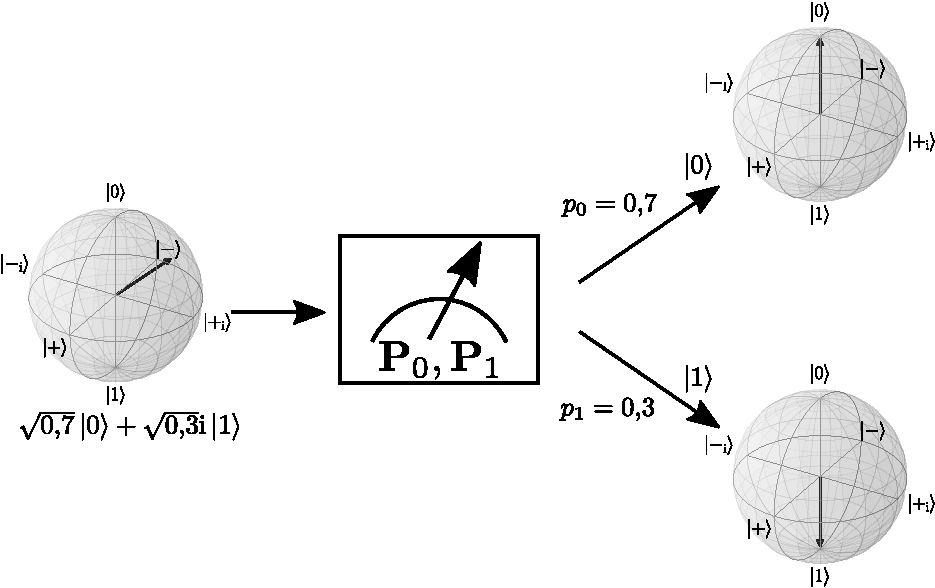
\includegraphics[height=0.38\textheight]{pics/pomiar_sz}}\\
	\subbottom[Pomiar z~wykorzystaniem macierzy $\mat{Q}_{-_\i}=\ketbra{-_\i}{-_\i}, \mat{Q}_{+_\i}=\ketbra{+_\i}{+_\i}$.\label{rys:pomiar-Q}]%
	{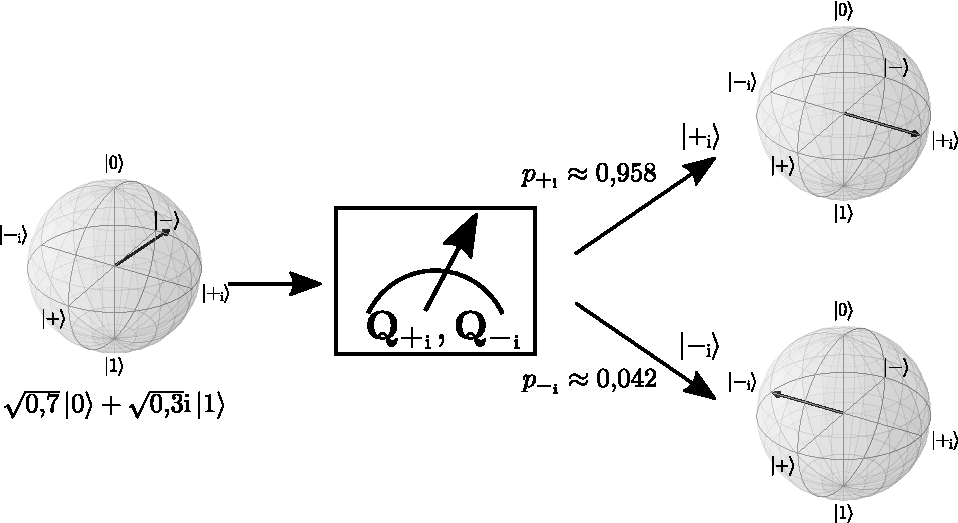
\includegraphics[height=0.38\textheight]{pics/pomiar_sy}}
	\caption{Schemat dwóch różnych pomiarów kwantowych tego samego stanu
		$\sqrt{0{,}7}\ket{0}+\sqrt{0{,}3}\i\ket{1}$. W~zależności od~rodzaju pomiaru
		uzyskujemy inne wyniki z~różnymi prawdopodobieństwami oraz~inne stany
		po~wykonaniu pomiaru.
		Takie zachowanie układów jest charakterystyczne dla~mechaniki kwantowej.
	}
	\label{rys:pomiar}
\end{figure}


\subsection{Szeregowanie pomiarów}
Tak~samo jak~bramki kwantowe, pomiary mogą być wykonywane jeden po~drugim.\index{pomiar!szeregowanie}
Oczywiście trzeba brać pod~uwagę, że~pierwszy pomiar zmieni stan kwantowy
i~wynik drugiego pomiaru będzie zależał od~wyniku pierwszego pomiaru.

Jeżeli~wykonujemy ten sam pomiar wielokrotnie, to wynik, który otrzymaliśmy
z~pierwszego pomiaru, otrzymamy też w~każdym następnym pomiarze. Weźmy zatem
pod~uwagę stan $\ket{\psi}$
oraz~pomiar
$$\mathcal{P}=\{\mat{P}_0,\mat{P}_1, \ldots, \mat{P}_{n-1}\}.$$
Jeżeli~dokonamy
pomiaru tego stanu jednokrotnie i~zmierzymy wynik $i$, to otrzymamy stan
$$
	\ket{\psi_i} = \frac{\mat{P}_i\ket{\psi}}{\norm{\mat{P}_i\ket{\psi}}}.
$$
Zmierzmy ten stan jeszcze raz i~zobaczmy, jakie jest prawdopodobieństwo zmierzenia wyniku $j$:
$$
	p_j'=\norm{\mat{P}_j\ket{\psi_i}}^2 = \norm{\frac{\mat{P}_j\mat{P}_i\ket{\psi}}{\norm{\mat{P}_i\ket{\psi}}}}^2.
$$
Ponieważ $\mat{P}_j \mat{P}_i$ jest równe $\mat{0}$ dla~różnych $i$ i~$j$, to prawdopodobieństwo
otrzymania za~drugim razem wyniku innego niż~za~pierwszym wynosi 0.
Natomiast prawdopodobieństwo otrzymania za~drugim razem tego samego wyniku co~za~pierwszym razem wynosi
$$
	p_i'=\norm{\frac{\mat{P}_i\mat{P}_i\ket{\psi}}{\norm{\mat{P}_i\ket{\psi}}}}^2 = \norm{\frac{\mat{P}_i\ket{\psi}}{\norm{\mat{P}_i\ket{\psi}}}}^2 =
	\frac{1}{\norm{\mat{P}_i\ket{\psi}}^2} \norm{\mat{P}_i\ket{\psi}}^2 = 1.
$$
Zatem widać, że~jeżeli~za~pierwszym razem wykonaliśmy pomiar
$\mathcal{P}$ na~stanie $\ket{\psi}$ i~otrzymaliśmy wynik~$i$ oraz~stan
po~pomiarze $\ket{\psi_i}$, to po~wykonaniu tego samego pomiaru raz
jeszcze na~otrzymanym stanie uzyskamy ten sam wynik~$i$. Zatem stan
$\ket{\psi_i}$ pozostanie niezmieniony.

\subsection{Pomiar częściowy stanu wielosystemowego}
Zobaczmy teraz, co się~dzieje, gdy~wykonamy pomiar częściowy stanu pierwszego
kubitu na~stanie złożonym z~dwóch kubitów. Przez \newterm{pomiar
	częściowy}\index{pomiar!częściowy} rozumiemy taki pomiar wykonywany na~układzie
wielu kubitów, że~na~części z~nich dokonujemy pomiaru trywialnego, a~na~części --
nietrywialnego.

Załóżmy, że~mamy do~dyspozycji stan
$$
	\ket{\psi} = \alpha_{00}\ket{00} + \alpha_{01}\ket{01} + \alpha_{10}\ket{10} + \alpha_{11}\ket{11}
$$
i~wykonujemy pomiar $\mathcal{P}=\{\mat{P}_0=\ketbra{0}{0},\mat{P}_1=\ketbra{1}{1}\}$
na~pierwszym kubicie oraz pomiar trywialny na drugim.
Wówczas wynik $0$ z~pomiaru pierwszego kubitu uzyskujemy z~prawdopodobieństwem
\begin{align*}
	p_{0?} & = \norm{\mat{P}_0\otimes\mat{\id}_? \ket{\psi}}^2 =
	\norm{\begin{bmatrix} 1 & 0 & 0 & 0 \\  0 & 1 & 0 & 0 \\  0 & 0 & 0 & 0 \\  0 & 0 & 0 & 0 \end{bmatrix}
		\begin{bmatrix} \alpha_{00} \\ \alpha_{01} \\ \alpha_{10} \\ \alpha_{11} \end{bmatrix}}^2 =
	\norm{\begin{bmatrix} \alpha_{00} \\ \alpha_{01} \\ 0 \\ 0 \end{bmatrix}}^2  =                       \\
	       & = \abs{\alpha_{00}}^2 + \abs{\alpha_{01}}^2.
\end{align*}
Odpowiednio wynik $1$ uzyskujemy z~prawdopodobieństwem $$p_{1?} = \abs{\alpha_{10}}^2 + \abs{\alpha_{11}}^2.$$
Stan po~zmierzeniu $0$ na~pierwszym kubicie staje~się
$$
	\ket{\psi_{0?}}=
	\frac{\alpha_{00}\ket{00} + \alpha_{01}\ket{01}}{\sqrt{|\alpha_{00}|^2 + |\alpha_{01}|^2}} =
	\ket{0}\otimes\frac{\alpha_{00}\ket{0} + \alpha_{01}\ket{0}}{\sqrt{|\alpha_{00}|^2 + |\alpha_{01}|^2}},
$$
a po~zmierzeniu $1$ -- staje~się
$$
	\ket{\psi_{1?}}=
	\frac{\alpha_{10}\ket{10} + \alpha_{11}\ket{11}}{\sqrt{|\alpha_{10}|^2 + |\alpha_{11}|^2}} =
	\ket{1}\otimes\frac{\alpha_{10}\ket{0} + \alpha_{11}\ket{1}}{\sqrt{|\alpha_{10}|^2 + |\alpha_{11}|^2}}.
$$

Zobaczmy, co się~stanie, gdy przeprowadzimy go na~stanie Bella
$\ket{\Phi^+}=\frac{1}{\sqrt{2}}(\ket{00}+\ket{11})$. Wówczas mamy
$\alpha_{00}=\alpha_{11}=\frac{1}{\sqrt{2}}$ oraz $\alpha_{01}=\alpha_{10}=0$. Zatem zmierzenie $0$
na~pierwszym kubicie da nam stan po~pomiarze $\ket{00}$, a~zmierzenie $1$ da nam
stan $\ket{11}$. Czyli~-- jak widać -- wynik pomiaru na~pierwszym kubicie determinuje
stan po~pomiarze drugiego kubitu, a~zatem również wynik pomiaru na~drugim. Efekt
taki jest utożsamiany ze~splątaniem kwantowym i~-- jako taki -- jest on bardzo istotny dla~informatyki kwantowej.

\section{Podsumowanie}
W~powyższym rozdziale wprowadziliśmy pojęcia stanu, bramki kwantowej i~pomiaru kwantowego. Dzięki temu wiemy teraz,
jak opisywane są układy kwantowe, jak zmieniają~się w~czasie i~jak są
odczytywane ich właściwości. W~komputerach i~systemach kwantowych te operacje wykonywane są
cyklicznie po~to, by~implementować protokoły lub~algorytmy kwantowe.


% LTeX: language=pl-PL
\chapter{Informatyka kwantowa}
\chapterauthor{PG}
% +Oskar Słowik w wydaniu 2

\section{Gra w~obracanie monety}
\subsection{Wersja klasyczna}
Wyobraźmy sobie następującą grę, w~której bierze udział dwoje graczy:
Eve i~Świadek Sądu Natury (zwany dalej Świadkiem)\footnote{Są to
	oczywiście bohaterowie naszego komiksu.}. Gracze mają do~dyspozycji
monetę, która jest zamknięta w~pudełku, więc~nie~mogą jej zobaczyć
w~trakcie gry; natomiast wiedzą, że~na~początku gry moneta jest
odwrócona orłem do~góry. Gra składa~się z~trzech ruchów: pierwszy
wykonuje Eve, drugi -- Świadek, trzeci -- znowu Eve. Ruch polega
na~odwróceniu monety bądź~pozostawieniu jej w~takim stanie, w~jakim
była. Oczywiście to, jaki ruch wykona jeden z~graczy, pozostaje
tajemnicą dla~drugiego. Po~dokonaniu ostatniego ruchu pudełko zostaje
otwarte i~gracze mogą sprawdzić, czy~moneta jest odwrócona orłem,
czy~reszką do~góry. Eve wygrywa, jeśli~moneta będzie w~pozycji
,,orzeł'', a~Świadek -- jeśli~w~pozycji ,,reszka''.

Łatwo sprawdzić, że~w grze w obracanie monety nie~istnieje strategia
wygrywająca dla~żadnego z~graczy i~najlepsze, co oboje mogą zrobić, to
wylosować swoje ruchy. Wtedy dla~każdego z~nich szansa na~wygraną wynosi
50\%.

\subsection{Wersja kwantowa}
Zastanówmy~się teraz, co się~stanie, jeżeli~gracze będą mieć do~dyspozycji nie~monetę,
ale~kubit.
Żeby~zamodelować taką sytuację, przypiszmy pozycji monety ,,orzeł'' stan $\ket{0}$ oraz~macierz
pomiaru $\mat{P}_0=\ketbra{0}{0}$, a~pozycji ,,reszka''
stan $\ket{1}$ i~macierz pomiaru $\mat{P}_1=\ketbra{1}{1}$. Obrócenie monety --
kubitu będzie wówczas odpowiadać bramce $\mat{X}$, a~pozostawienie go w~stanie, w~jakim był
-- bramce $\mat{\id}$. W~tym schemacie ruchom wykonywanym przez~graczy odpowiada czynność nałożenia bramki
kwantowej na~kubit -- za~pierwszym i~trzecim razem przez~Eve, a~za~drugim -- przez~Świadka.
Otworzeniu pudełka odpowiada pomiar kwantowy.
Przykładową rozgrywkę można zatem zapisać w~następujący sposób:

Stan początkowy to
$$
	\ket{\psi_{t=0}}=\ket{0}.
$$
Eve decyduje się nic nie~robić:
$$
	\ket{\psi_{t=1}}=\mat{\id}\ket{0}=\ket{0}.
$$
Świadek decyduje~się obrócić kubit:
$$
	\ket{\psi_{t=2}}=\mat{X}\ket{0}=\ket{1}.
$$
Eve ponownie decyduje~się nic nie~robić:
$$
	\ket{\psi_{t=3}}=\mat{\id}\ket{1}=\ket{1}.
$$
Gracze dokonują pomiaru $\{\mat{P}_0,\mat{P}_1\}$ i~otrzymują
prawdopodobieństwa zmierzenia ,,orła'' -- wyniku pomiaru~$0$ -- lub~,,reszki'' -- wyniku pomiaru~$1$
$$
	p_0=\norm{\ketbra{0}{0}\ket{1}}=0, \quad p_1=\norm{\ketbra{1}{1}\ket{1}}=1.
$$
Zatem Świadek wygrywa z~prawdopodobieństwem $1$. Nie znaczy~to, że~Świadek wygrywa
tę~grę zawsze, a tylko tyle, że~wygrywa w~przypadku takiego ciągu ruchów.
Jeśli ciąg ruchów będzie inny, np.~$\mat{X}$, $\mat{X}$, $\mat{I}$, może wygrać Eve.

Dajmy teraz Eve przewagę: ona będzie wiedzieć, że~grają na~kubicie, a~Świadek nie~będzie tego świadom.
Zobaczmy teraz, co może zrobić Eve, jeżeli~wie, że~gra odbywa~się z~wykorzystaniem nie~monety, ale~kubitu.
Nasz stan początkowy to znowu:
$$
	\ket{\psi_{t=0}}=\ket{0}.
$$
Eve decyduje~się użyć ,,tajnego'' ruchu kwantowego i~nakłada bramkę Hadamarda:
$$
	\ket{\psi_{t=1}}=\mat{H}\ket{0}=\frac{1}{\sqrt{2}}\left(\ket{0}+\ket{1}\right).
$$
Załóżmy, że~Świadek decyduje~się obrócić kubit:
$$
	\ket{\psi_{t=2}}=\mat{X}\frac{1}{\sqrt{2}}\left(\ket{0}+\ket{1}\right)=\frac{1}{\sqrt{2}}\left(\ket{0}+\ket{1}\right).
$$
Jak widać, jego działanie nie~zmienia teraz stanu kubitu. Zatem niezależnie od~tego, czy~nakłada on bramkę $\mat{X}$ lub~$\mat{\id}$, nie~zmieni stanu kubitu.
Następnie Eve znowu nakłada bramkę Hadamarda:
\begin{equation*}
	\begin{split}
		\ket{\psi_{t=3}}=&\mat{H}\frac{1}{\sqrt{2}}\left(\ket{0}+\ket{1}\right)=
		\frac{1}{\sqrt{2}}\left(\mat{H}\ket{0}+\mat{H}\ket{1}\right)=\\
		=&\frac{1}{\sqrt{2}}\left(\frac{1}{\sqrt{2}}\left(\ket{0}+\ket{1}\right)+
		\frac{1}{\sqrt{2}}\left(\ket{0}-\ket{1}\right)\right)=\\
		=&\frac{1}{2}\left(\ket{0}+\ket{1}+\ket{0}-\ket{1}\right)=
		\ket{0}
	\end{split}
\end{equation*}
Gracze dokonują pomiaru $\{\mat{P}_0,\mat{P}_1\}$ i~otrzymują prawdopodobieństwa
$$
	p_0=\norm{\ketbra{0}{0}\ket{0}}=1, \quad p_1=\norm{\ketbra{1}{1}\ket{1}}=0.
$$
W~efekcie Eve wygrywa, i~to wygrywa niezależnie od~działań Świadka.
Zatem możliwość wykorzystania większej liczby bramek kwantowych -- zwłaszcza takich,
które nie mają odpowiedników klasycznych -- daje przewagę jednemu z~graczy.
Na końcu tego rozdziału umieszczon jest krótka
historyjka obrazkowa, która wyjaśnai jak Eve wygrała ze Świadkiem.

\section{Twierdzenie o~zakazie klonowania}
Możliwość kopiowania informacji zakodowanej w~postaci ciągów bitów wydaje~się być oczywista.
Gdy używamy komputerów w~życiu codziennym, ciągle kopiujemy strony www z~serwerów na~nasze urządzenia,
kopiujemy programy z~dysku komputera do~pamięci operacyjnej lub~po~prostu kopiujemy zdjęcia dla~znajomych i~rodziny.

Informacja zapisana w~postaci kubitów jest inna. Nie~można jej skopiować. Właściwość tę opisuje
twierdzenie o~zakazie klonowania, które można przedstawić dla~kubitów w~sposób opisany poniżej.

Wyobraźmy sobie, że~dana jest pewna bramka kwantowa $\mat{U_c}$ działającą
na~dwóch układach kwantowych, która dla~dowolnego stanu $\ket{\psi}$
działa następująco:
$$
	\ket{\psi}\otimes \ket{\psi} = \mat{U_c} (\ket{\psi}\otimes\ket{0}).
$$
Oznacza to, że~kopiuje ona nieznany stan $\ket{\psi}$ z~układu pierwszego na~układ drugi.
Weźmy zatem dwa dowolne stany $\ket{\psi_1}$ oraz~$\ket{\psi_2}$ i~zapiszmy dla~nich powyższe równanie:
\begin{eqnarray}
	\ket{\psi_1}\otimes \ket{\psi_1} &=& \mat{U_c} (\ket{\psi_1}\otimes\ket{0}),\nonumber\\
	\ket{\psi_2}\otimes \ket{\psi_2} &=& \mat{U_c} (\ket{\psi_2}\otimes\ket{0}).\nonumber
\end{eqnarray}
Policzmy teraz iloczyn skalarnym pomiędzy~wektorami w~górnym i~dolnym równaniu:
$$
	(\bra{\psi_1}\otimes \bra{\psi_1})(\ket{\psi_2}\otimes \ket{\psi_2}) =  (\bra{\psi_1}\otimes\bra{0}) \mat{U_c}^\dagger \mat{U_c} (\ket{\psi_2}\otimes\ket{0}).
$$
Ponieważ $\mat{U_c}$ jest macierzą unitarną, możemy usunąć z~równania $\mat{U_c}^\dagger \mat{U_c} =\mat{\id}$, a~następnie pogrupować składniki:
$$
	\braket{\psi_1}{\psi_2} \otimes \braket{\psi_1}{\psi_2} =  \braket{\psi_1}{\psi_2}\otimes\braket{0}{0}.
$$
Oczywiście $\braket{0}{0}=1$, a~iloczyn Kroneckera liczb jest równy iloczynowi tych liczb -- zatem otrzymujemy:
$$
	\braket{\psi_1}{\psi_2}^2 = \braket{\psi_1}{\psi_2}.
$$
To równanie ma dwa rozwiązania -- dla~$\braket{\psi_1}{\psi_2}=0$, czyli~wektorów
ortonormalnych, oraz~$\braket{\psi_1}{\psi_2}=1$, czyli~dla~wektorów $\ket{\psi_1}=\ket{\psi_2}$.
Wynika z~tego, że~możemy klonować stany tylko z~ortonormalnego zbioru stanów. Ponieważ
zbiór wszystkich stanów nie~jest ortonormalny, zatem nie~istnieje bramka unitarna,
która pozwalałaby na~klonowanie dowolnych stanów.

Twierdzenie to będzie nam potrzebne do~zrozumienia podstaw działania kwantowego
protokołu dystrybucji klucza kwantowego -- podstawy kwantowej kryptografii --
oraz~zamków kwantowych.

\section{Zamki kwantowe}
Jak widać, klonowanie dowolnych stanów kwantowych jest niemożliwe. Można więc~wyobrazić
sobie proste zastosowanie tego faktu do~tworzenia niepodrabialnych
kluczy do~zamków.

Wyobraźmy sobie klucz, który składa~się z~$n$ kubitów, oraz~zamek\index{zamek kwantowy}, który zawiera
urządzenie elektroniczne, a~także kwantowe urządzenie pomiarowe, które umie zmierzyć
stan klucza. Zamek może zostać otwarty przez~odpowiedni klucz
i~nie~powinien być otwierany przez~inny klucz.

Załóżmy teraz, że~dany jest ciąg kubitów
$
	\ket{\psi_1},\ket{\psi_2},\ldots,\ket{\psi_n},
$
które stanowią klucz.
Chcemy, aby~każdy kubit był w~jednym z~następujących stanów:
$$
	\ket{0}, \ket{1}, \ket{+}=\frac{1}{\sqrt{2}}(\ket{0}+\ket{1}) \text{ lub } \ket{-}=\frac{1}{\sqrt{2}}(\ket{0}-\ket{1}).
$$

Aby~zbudować mechanizm zamka, potrzebujemy dwóch pomiarów:
\begin{itemize}
	\item pierwszego $\mathcal{P}=\{\mat{P}_0=\ketbra{0}{0}, \mat{P}_1=\ketbra{1}{1}\}$
	\item i~drugiego
	      $\mathcal{Q}=\{\mat{Q}_+=\ketbra{+}{+}, \mat{Q}_-=\ketbra{-}{-}\}$.
\end{itemize}
Wyniki pierwszego pomiaru
będziemy oznaczać jako~$0$ i~$1$, a~wyniki drugiego pomiaru będziemy oznaczać jako~$+$ i~$-$. Od~razu widać, że~pomiar
$\mathcal{P}$ jest dopasowany do~stanów $\ket{0}$ i~$\ket{1}$ i~potrafi
je doskonale rozróżniać, co~znaczy, że~dla stanu $\ket{0}$ zwróci zawsze wynik
$0$, a~dla~stanu $\ket{1}$ zawsze zwróci wynik $1$. Natomiast dla~stanów
$\ket{+}$ i~$\ket{-}$ zwróci wyniki $0$ lub~$1$ z~prawdopodobieństwem
$\frac{1}{2}$. Podobnie będzie w~przypadku pomiaru~$\mathcal{Q}$: jest
on~dopasowany do~stanów $\ket{+}$ i~$\ket{-}$, które rozróżnia doskonale,
ale dla stanów $\ket{0}$ i~$\ket{1}$ zwraca wyniki $+$ i~$-$ z~prawdopodobieństwem~$\frac{1}{2}$.

Zatem jeżeli~mechanizm zamka zna stany kubitów klucza, to może dokonywać
odpowiednich dopasowanych pomiarów na~ich stanach. Jeżeli~przynajmniej jeden pomiar zwróci
wynik, który nie~jest oczekiwany, to znaczy, że~klucz nie~pasuje do~zamka.

Co się~więc~stanie, jeżeli~ktoś, kto zdobyłby klucz, zechce go~podrobić?
Zakładamy, że~osoba, która podrabia klucz, nie~wie nic na~temat tego, jakie pomiary są
przeprowadzane w~zamku, i~oczywiście nie~wie nic o~stanach klucza. Zatem jedyne, co może zrobić,
to wybrać losowo pomiary i~zmierzyć stany kubitów klucza. Wtedy z~prawdopodobieństwem
$\frac{1}{2}$ wybierze pomiar, który jest dopasowany do~stanu kubitu zamka.
Jeżeli~zostanie wybrany niewłaściwy pomiar, to zamek wykryje błąd z~prawdopodobieństwem
$\frac{1}{2}$. Zatem kubit podrobionego klucza zostanie poprawnie
rozpoznany przez~zamek z~prawdopodobieństwem $\frac{3}{4}$ (zobacz Rysunek~\ref{rys:zamek}).
Jeżeli~klucz będzie się~składał z~$n$ kubitów, to prawdopodobieństwo otwarcia
zamka podrobionym kluczem wynosi $\left(\frac{3}{4}\right)^n$ -- czyli~maleje
wraz~ze~wzrostem liczby kubitów i~dla~dużej liczby kubitów jest bardzo małe.

\begin{figure}[h]
	\centering
	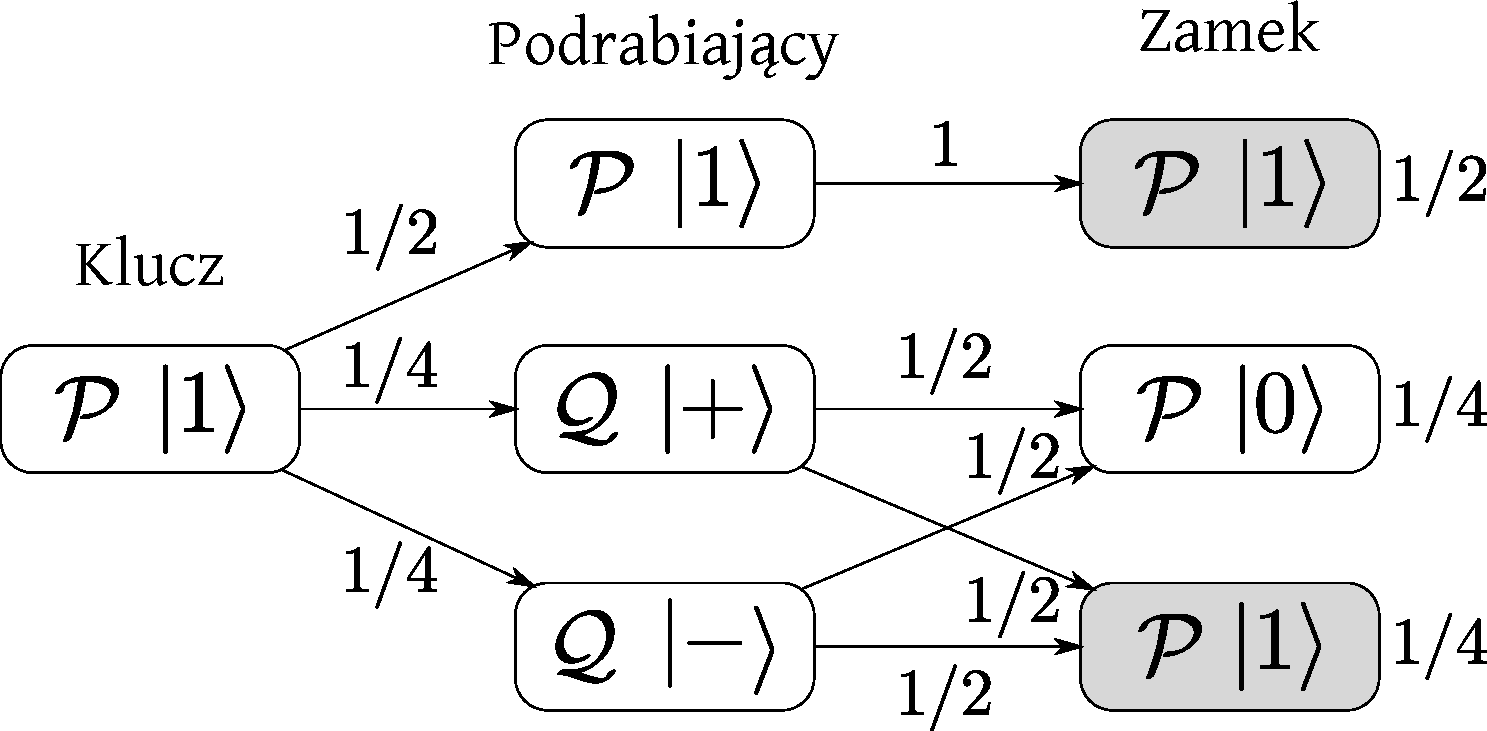
\includegraphics[width=0.7\textwidth]{pics/zamekkwantowy}
	\caption{Schemat obliczania prawdopodobieństwa prawidłowego
		zmierzenia stanu kubitu podrobionego klucza. Kolorem szarym oznaczono
		pomiary, które wykonuje zamek i~które zwrócą oczekiwany wynik.}
	\label{rys:zamek}
\end{figure}


Jak widać, nie jest łatwo podrobić klucze kwantowe. Czy~jednak istnieje
możliwość ich wykradzenia? Tego dowiemy się pod~koniec niniejszego rozdziału.

\section{Kwantowa dystrybucja klucza}
Wyobraźmy sobie, że~istnieją dwie osoby oddalone od~siebie fizycznie,
które chcą przesłać pomiędzy sobą pewną informację w~postaci ciągu
bitów. Informacja ta jest tajna i~nie powinna zostać przechwycona
przez~osoby trzecie\index{kwantowa dystrybucja klucza}. Powiedzmy, że
podmiotem nadającym informację jest Biblioteka Orbitalna Aleksandria
(zwana dalej Aleksandrią), odbierającym -- Centrum Komunikacji Kwantowej
(zwane dalej Centrum), a~osobą próbującą przechwycić informację -- Eve.

Klasyczne rozwiązanie tego problemu polega na~wykorzystaniu któregoś
z~algorytmów szyfrujących oraz~klasycznego kanału informacyjnego. Wadą tego
rozwiązania jest to, że~nie~mamy pewności, czy~algorytmy szyfrujące na~pewno są
bezpieczne. Nasza wiara w~ich bezpieczeństwo wynika tylko~i~wyłącznie
z~przekonania, że~nie~wiadomo, w~jaki sposób szybko i~efektywnie wykonywać pewne
algorytmy, takie jak~np.~algorytm znajdowania dzielników liczb.

\subsection{Szyfr Vernama}
Istnieje szyfr pozwalający przesyłać informację całkowicie bezpiecznie.
Jest to~szyfr Vernama\footnote{Od~nazwiska amerykańskiego inżyniera Gilberta Vernama
	(1890 -- 1960).}\index{szyfr Vernama}. Jego idea jest bardzo prosta.
Aleksandria i~Centrum
współdzielą pewien tylko sobie znany ciąg losowych bitów, czyli~klucz. Zakładamy,
że~Aleksandria chce przesłać tajną wiadomość w~postaci binarnej do~Centrum. Ażeby~ukryć
tę wiadomość przed~Eve, dla~każdego bitu wiadomości wykonuje operację XOR
z~odpowiednim bitem klucza. W~ten~sposób uzyskuje szyfrogram, który wysyła do~Centrum.
Po~otrzymaniu zaszyfrowanej wiadomości Centrum odwraca działanie Aleksandrii -- tzn.~wykonuje operację XOR na~każdym
bicie szyfrogramu z~odpowiednim bitem klucza, i~w~ten sposób odzyskuje oryginalną wiadomość
nadaną przez~Aleksandrię.

Operacja XOR działa na~dwóch bitach następująco: jeżeli~oba bity są różne, to
zwraca $1$, jeżeli~są równe -- to zwraca $0$.
Możemy zatem stworzyć Tabelę~\ref{tab:xor} wejść i~wyjść operacji XOR, w~której
dwie lewe kolumny odpowiadają argumentom operacji (wejściom), a~prawa kolumna
odpowiada wartościom (wyjściu).

\begin{table}[h!]
	\centering
	\begin{tabular}{ccc}
		$\text{we}_1$ & $\text{we}_2$ & $\text{wy}$ \\
		\toprule
		0             & 0             & 0           \\
		0             & 1             & 1           \\
		1             & 0             & 1           \\
		1             & 1             & 0
	\end{tabular}
	\caption{Tabela argumentów i~wartości operacji $\text{wy}=XOR(\text{we}_1, \text{we}_2)$}
	\label{tab:xor}
\end{table}

Oznaczmy zatem tajną wiadomość Aleksandrii jako ciąg bitów $$a_1, a_2, \ldots, a_n,$$
szyfrogram jako $$s_1, s_2, \ldots, s_n,$$ klucz jako $$k_1, k_2,
	\ldots, k_n,$$ a~wiadomość odczytaną przez~Centrum jako $$b_1, b_2, \ldots, b_n.$$
Wówczas w~procesie szyfrowania uzyskujemy szyfrogram ze~wzoru $s_i=XOR(a_i, k_i)$ dla~każdego
$i=1,2,\ldots,n$. Centrum natomiast deszyfruje wiadomość, korzystając ze~wzoru
$b_i=XOR(s_i, k_i)$. Łatwo można sprawdzić, że~dla~każdego $i=1,2,\ldots,n$ $a_i
	= b_i$, co oznacza, że~wiadomość otrzymana przez~Centrum jest tą, którą nadała Aleksandria.
Przykład takiego procesu szyfrowania i~deszyfrowania jest pokazany na~Rysunku~\ref{rys:vernam}.

\begin{figure}[h]
	\centering
	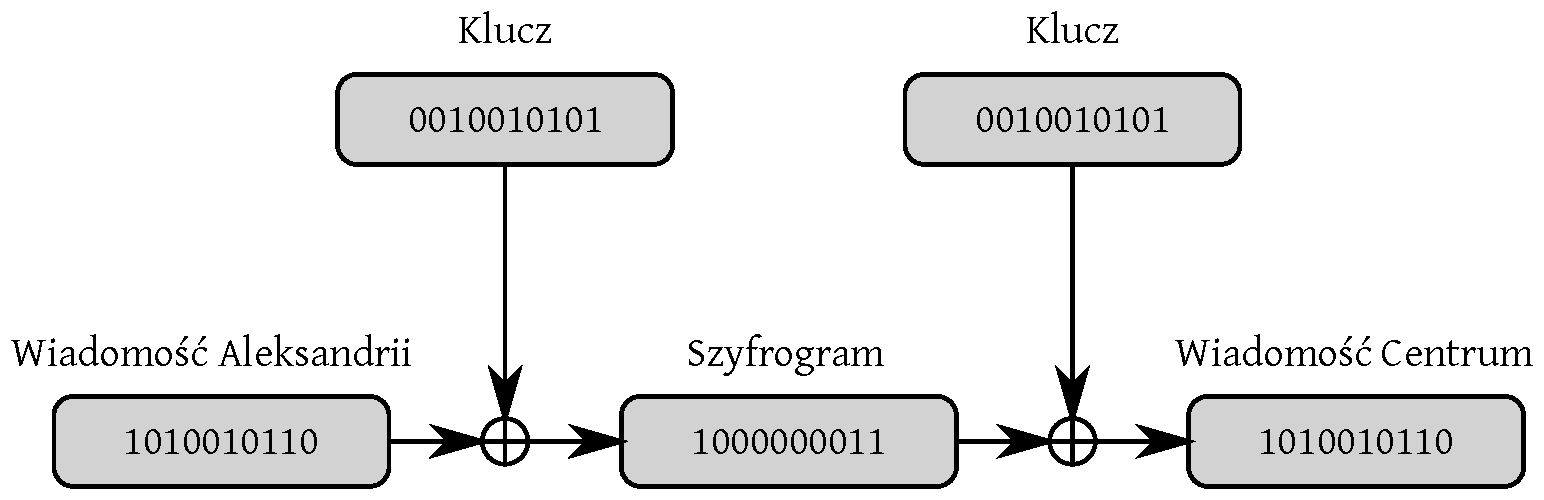
\includegraphics[width=0.7\linewidth]{pics/vernam}
	\caption{Przykład działania szyfru Vernama. Symbol $\oplus$ oznacza operację XOR.}
	\label{rys:vernam}
\end{figure}

Jeżeli~klucz jest całkowicie losowy, to~dla~Eve, która nie~zna klucza, szyfrogram
także jest całkowicie losowy i~nie~niesie żadnej informacji o~tajnej wiadomości.

\subsection{Protokół BB84}
Szyfr Vernama ma pewną wadę -- wymaga~on~tego, by~nadawca i~odbiorca wiadomości
korzystali z~klucza kryptograficznego, który ma długość samej wiadomości oraz~jest~całkowicie
losowy. Taki klucz -- po pierwsze -- trudno stworzyć, ponieważ nie~jest łatwo
wylosować całkowicie losowy ciąg bitów; a~po~drugie -- dystrybuować pomiędzy
nadawcę i~odbiorcę. Rozwiązaniem
problemu losowania i~dystrybucji klucza jest protokół
BB84\footnote{Zaproponowany w~roku 1984 przez Charlesa Bennetta i~Gilles'a
	Brassarda.}, który wykorzystuje kubity i~mechanikę kwantową
do~przygotowania i~dystrybucji klucza kryptograficznego.

Podobnie jak~w~konstrukcji zamków i~kluczy kwantowych, w~protokole BB84 używamy
czterech stanów jednokubitowych
$$
	\ket{0}, \ket{1}, \ket{+}=\frac{1}{\sqrt{2}}(\ket{0}+\ket{1})
	\text{ lub } \ket{-}=\frac{1}{\sqrt{2}}(\ket{0}-\ket{1})
$$
oraz~dwóch rodzajów pomiarów
$\mathcal{P}=\{\mat{P}_0=\ketbra{0}{0}, \mat{P}_1=\ketbra{1}{1}\}$ i
$\mathcal{Q}=\{\mat{Q}_+=\ketbra{+}{+}, \mat{Q}_-\ketbra{-}{-}\}$.

Aleksandria -- nadawca -- nadaje kubity w~stanach wymienionych powyżej, natomiast Centrum
-- odbiorca -- wykonuje wymienione powyżej pomiary. Zależność wyniku
pomiaru od~wysłanego stanu kubitu i~od~tego, jaki pomiar został na~nim dokonany, przedstawia
Tabela~\ref{tab:bb84}.

\begin{table}[h]
	\begin{center}
		\begin{tabular}{llc}
			stan      & pomiar        & wynik pomiaru                       \\
			\toprule
			$\ket{0}$ & $\mathcal{P}$ & $0$                                 \\
			\midrule
			$\ket{1}$ & $\mathcal{P}$ & $1$                                 \\
			\midrule
			$\ket{+}$ & $\mathcal{Q}$ & $+$                                 \\
			\midrule
			$\ket{-}$ & $\mathcal{Q}$ & $-$                                 \\
			\midrule
			$\ket{0}$ & $\mathcal{Q}$ & $+$ lub $-$ z $p_+=p_-=\frac{1}{2}$ \\
			\midrule
			$\ket{1}$ & $\mathcal{Q}$ & $+$ lub $-$ z $p_+=p_-=\frac{1}{2}$ \\
			\midrule
			$\ket{+}$ & $\mathcal{P}$ & $0$ lub $1$ z $p_0=p_1=\frac{1}{2}$ \\
			\midrule
			$\ket{-}$ & $\mathcal{P}$ & $0$ lub $1$ z $p_0=p_1=\frac{1}{2}$ \\
		\end{tabular}
		\caption{Zależność wyniku pomiaru od~stanu i~wybranego rodzaju pomiaru.}
		\label{tab:bb84}
	\end{center}
\end{table}

Jeżeli~stan nadawany przez~Aleksandrię nie~jest dopasowany do~pomiaru,
to wynik pomiaru tego stanu jest losowy, co~pokazują ostatnie cztery wiersze
tabeli. Dodatkowo po~pomiarze stan początkowy zmienia~się na~stan
odpowiadający wynikowi pomiaru. Fakt ten można wykorzystać do~wykrywania
podsłuchu podczas~przesyłania kubitów. Pozwala to na~stworzenie
protokołu dystrybucji kluczy kwantowych składającego~się z~poniższych
kroków:

\paragraph{Krok 1} Aleksandria wysyła sekwencję kubitów, z~których każdy jest w~losowo
i~niezależnie wybranym stanie: $\ket{0}$, $\ket{1}$,
$\ket{+}=\frac{\ket{0}+\ket{1}}{\sqrt{2}}$ lub~$\ket{-}=\frac{\ket{0}-\ket{1}}{\sqrt{2}}$.
\paragraph{Krok 2} Centrum dokonuje -- również losowo i~niezależnie --
wyboru, który z~dwóch pomiarów -- $\mathcal{P}$ lub~$\mathcal{Q}$ -- przeprowadzi na~każdym z~kubitów z~osobna.
\paragraph{Krok 3} Centrum zapisuje swój wybór i~wyniki pomiarów.
\paragraph{Krok 4} Centrum wysyła do~Aleksandrii w~sposób jawny swój wybór pomiarów.
\paragraph{Krok 5} Aleksandria przekazuje Centrum informację, które pomiary były dopasowane do stanów
nadanych kubitów.
\paragraph{Krok 6} Aleksandria i~Centrum dzielą kubity na~dwie części: jedna zawiera te, które
zostały zmierzone za~pomocą dopasowanego pomiaru, a~druga -- te, które nie~zostały zmierzone w~ten~sposób.

Możemy zauważyć, że~średnio w~połowie przypadków został użyty
niedopasowany pomiar. Przypadki te muszą zostać odrzucone, gdyż~wynik
niedopasowanego pomiaru jest całkowicie losowy.

Jeżeli~nie~zaistniały przekłamania i~nikt nie~ingerował w~proces
transmisji, to ok.~50\% kubitów zmierzonych przez~Centrum ma ten sam  stan, który został nadany w~Kroku 1 przez Aleksandrię. Te właśnie kubity można wykorzystać do~stworzenia klucza kryptograficznego.

\paragraph{Krok 7} Aleksandria i~Centrum wybierają pewien wspólny
podzbiór kubitów spośród tych, które zostały zmierzone przy~użyciu
dopasowanego pomiaru, i~w~sposób jawny je porównują. Kubity te oczywiście
będzie trzeba odrzucić, jako że~zostały ujawnione.

Jeżeli~nie~doszło do~podsłuchania transmisji kubitów, to porównanie
powinno dać całkowicie zgodne wyniki. Wówczas Aleksandria i~Centrum
przypisują stanom $\ket{0}$, $\ket{-}$ bit $0$, a~stanom $\ket{1}$,
$\ket{+}$ bit $1$. Zatem teraz Aleksandria i~Centrum mają wspólny
losowy klucz kryptograficzny, którego mogą użyć do~przekazania sobie
zaszyfrowanej szyfrem Vernama wiadomości.

Jeżeli~podczas wykonywania protokołu Aleksandria i~Centrum wykryły
jakiekolwiek niezgodności, oznacza to, że~kubity zostały już~poddane
pomiarowi przez~osobę trzecią i~nie~należy ich używać do~tworzenia
klucza. W~takim przypadku muszą zaniechać przesyłania tajnej informacji.

Zastanówmy~się, jakie próby ataku może podjąć Eve. Nie~może skopiować
stanu kubitu i~zmierzyć jego kopii, gdyż~tego zabrania twierdzenie
o~zakazie klonowania. Może natomiast wpiąć~się do~kwantowego kanału
transmisji i~przechwytywać wszystkie kubity nadesłane przez~Aleksandrię,
dokonywać na~nich pomiaru i~następnie odsyłać do~Centrum. Taka technika
podsłuchu jest bardzo łatwa do~zdemaskowania, ponieważ skoro Eve nie wie, jakie
kubity zostały nadane, nie~wie też, jaki pomiar powinna wybrać. Jeśli więc Eve wybierze
niewłaściwy pomiar, doprowadzi do~zmiany stanów kubitów, co --
po~wymianie klucza -- Aleksandria i~Centrum z~łatwością wykryją. Eve
może również przechwytywać tylko niektóre kubity i~je mierzyć, ale~wtedy
nie~uzyska całego klucza kryptograficznego, a~jej działanie też~może
zostać wykryte.

Tabela~\ref{tab:bb84przyklad} pokazuje, jak może przebiegać krótki
proces ustalania klucza przez Aleksandrię i~Centrum, gdy~Eve
nie~podsłuchuje. Natomiast w~Tabeli~\ref{tab:bb84przykladzewą} pokazano,
co się~dzieje, gdy~Eve podsłuchuje komunikację kwantową.

\definecolor{Gray}{gray}{0.9}
\def\colw{0.7em}
\newcolumntype{P}[1]{>{\centering\arraybackslash}p{#1}}
\newcolumntype{g}{>{\columncolor{Gray}}P{\colw}}
\newcolumntype{w}{P{\colw}}
\begin{table}[h]
	\resizebox{\textwidth}{!}{
		\centering
		\tiny
		\begin{tabular}{l|gggwwwgwgwwgwgwwwggg}
			$A_1$ & $\ket{0}$     & $\ket{1}$     & $\ket{1}$     & $\ket{+}$     & $\ket{1}$     & $\ket{+}$     & $\ket{+}$     & $\ket{-}$     & $\ket{-}$     & $\ket{0}$     & $\ket{0}$     & $\ket{-}$     & $\ket{-}$     & $\ket{1}$     & $\ket{0}$     & $\ket{1}$     & $\ket{+}$     & $\ket{1}$     & $\ket{0}$     & $\ket{0}$     \\
			$C_1$ & $\mathcal{P}$ & $\mathcal{P}$ & $\mathcal{P}$ & $\mathcal{P}$ & $\mathcal{Q}$ & $\mathcal{P}$ & $\mathcal{Q}$ & $\mathcal{P}$ & $\mathcal{Q}$ & $\mathcal{Q}$ & $\mathcal{Q}$ & $\mathcal{Q}$ & $\mathcal{P}$ & $\mathcal{P}$ & $\mathcal{Q}$ & $\mathcal{Q}$ & $\mathcal{P}$ & $\mathcal{P}$ & $\mathcal{P}$ & $\mathcal{P}$ \\
			$C_2$ & $\ket{0}$     & $\ket{1}$     & $\ket{1}$     & $\ket{1}$     & $\ket{-}$     & $\ket{0}$     & $\ket{+}$     & $\ket{0}$     & $\ket{-}$     & $\ket{+}$     & $\ket{-}$     & $\ket{-}$     & $\ket{1}$     & $\ket{1}$     & $\ket{-}$     & $\ket{-}$     & $\ket{0}$     & $\ket{1}$     & $\ket{0}$     & $\ket{0}$     \\
			bit   & 0             & 1             & 1             &               &               &               & 1             &               & 0             &               &               & 0             &               & 1             &               &               &               & 1             & 0             & 0
		\end{tabular}
	}
	\caption{Przykład realizacji protokołu BB84 bez~podsłuchu. Oznaczenia wierszy:
		$A_1$ -- stany wysłane przez~Aleksandrię,
		$C_1$ -- pomiary wybrane przez~Centrum,
		$C_2$ -- stany po~pomiarze Centrum,
		bit -- bit klucza.
		Kolumny oznaczone na~szaro wyróżniają przypadki, dla~których stan kubitu
		nadanego przez~Aleksandrię pokrywa~się z~kubitem zmierzonym przez~Centrum. We~wszystkich
		przypadkach, w~których Aleksandria nadała kubit w~stanie dopasowanym do~pomiaru Centrum, Centrum zmierzyło
		odpowiedni stan -- zatem Aleksandria i~Centrum nie~mają powodu podejrzewać, że~ktoś podsłuchiwał
		ustalanie klucza.
	}
	\label{tab:bb84przyklad}
\end{table}

\begin{table}[h]
	\resizebox{\textwidth}{!}{
		\centering\tiny
		\begin{tabular}{l|wwwwgwwgwwwwgwwgwwww}
			$A_1$ & $\ket{0}$     & $\ket{1}$     & $\ket{1}$     & $\ket{+}$     & $\ket{1}$     & $\ket{+}$     & $\ket{+}$     & $\ket{-}$     & $\ket{-}$     & $\ket{0}$     & $\ket{0}$     & $\ket{-}$     & $\ket{-}$     & $\ket{1}$     & $\ket{0}$     & $\ket{1}$     & $\ket{+}$     & $\ket{1}$     & $\ket{0}$     & $\ket{0}$     \\
			$E_1$ & $\mathcal{P}$ & $\mathcal{P}$ & $\mathcal{Q}$ & $\mathcal{P}$ & $\mathcal{Q}$ & $\mathcal{P}$ & $\mathcal{Q}$ & $\mathcal{P}$ & $\mathcal{Q}$ & $\mathcal{Q}$ & $\mathcal{Q}$ & $\mathcal{Q}$ & $\mathcal{P}$ & $\mathcal{P}$ & $\mathcal{Q}$ & $\mathcal{Q}$ & $\mathcal{P}$ & $\mathcal{P}$ & $\mathcal{P}$ & $\mathcal{P}$ \\
			$E_2$ & $\ket{0}$     & $\ket{1}$     & $\ket{+}$     & $\ket{1}$     & $\ket{-}$     & $\ket{0}$     & $\ket{+}$     & $\ket{0}$     & $\ket{-}$     & $\ket{+}$     & $\ket{-}$     & $\ket{-}$     & $\ket{1}$     & $\ket{1}$     & $\ket{-}$     & $\ket{-}$     & $\ket{0}$     & $\ket{1}$     & $\ket{0}$     & $\ket{0}$     \\
			$C_1$ & $\mathcal{Q}$ & $\mathcal{P}$ & $\mathcal{P}$ & $\mathcal{P}$ & $\mathcal{P}$ & $\mathcal{P}$ & $\mathcal{Q}$ & $\mathcal{Q}$ & $\mathcal{Q}$ & $\mathcal{Q}$ & $\mathcal{Q}$ & $\mathcal{Q}$ & $\mathcal{Q}$ & $\mathcal{P}$ & $\mathcal{Q}$ & $\mathcal{P}$ & $\mathcal{P}$ & $\mathcal{P}$ & $\mathcal{Q}$ & $\mathcal{Q}$ \\
			$C_2$ & $\ket{+}$     & $\ket{1}$     & $\ket{1}$     & $\ket{1}$     & $\ket{0}$     & $\ket{0}$     & $\ket{+}$     & $\ket{+}$     & $\ket{-}$     & $\ket{+}$     & $\ket{-}$     & $\ket{-}$     & $\ket{+}$     & $\ket{1}$     & $\ket{-}$     & $\ket{0}$     & $\ket{0}$     & $\ket{1}$     & $\ket{+}$     & $\ket{+}$
		\end{tabular}
	}
	\caption{
		Przykład realizacji protokołu BB84 z~podsłuchem. Oznaczenia wierszy:
		$A_1$ -- stany wysłane przez~Aleksandrię,
		$E_1$ -- pomiary wybrane przez~Eve,
		$E_2$ -- stany po~pomiarze Eve,
		$C_1$ -- pomiary wybrane przez~Centrum,
		$C_2$ -- stany po~pomiarze Centrum.
		Kolumny oznaczone na~szaro wyróżniają przypadki, dla~których stan kubitu
		nadanego przez~Aleksandrię nie~pokrywa~się z~kubitem zmierzonym przez~Centrum. Te przypadki wskazują Aleksandrii i~Centrum, że~mogło dojść do~podsłuchu.
	}
	\label{tab:bb84przykladzewą}
\end{table}

Bezpieczeństwo protokołu BB84 zależy od~naszej ufności w~skuteczność
mechaniki kwantowej -- najlepiej potwierdzonej współczesnej teorii
fizycznej -- w~przeciwieństwie do~klasycznych protokołów kryptografii
asymetrycznej, w~przypadku której musimy zakładać, że~nikt nie~zna
skutecznych metod faktoryzacji liczb lub~liczenia logarytmu dyskretnego.

\section{Teleportacja kwantowa}
Rozważmy trzy osoby\footnote{Zwykle w protokole teleportacji myślimy o
	dwóch osobach -- jednej z dwoma kubitami, która chce przesłać informację,
	i drugiej z jednym kubitem, która jest odbiorcą.} -- Bretta, Eve i
Roberta. Każde z nich ma do dyspozycji jeden kubit. Wyobraźmy sobie, że
kubit~Bretta jest w nieznanym stanie, a Eve chce przesłać stan kubitu
Bretta do Roberta. Eve może zbliżyć swój kubit do kubitu Bretta, jednak
nie~ma możliwości przesłania do~Roberta informacji kwantowej --
tzn.~stanów kwantowych. Może do~niego natomiast przesłać informację
klasyczną. Jeśli~ma~do~dyspozycji tylko jedną kopię stanu, jest to oczywiście
niemożliwe. Natomiast jeżeli~Eve i~Robert współdzielą splątany stan
Bella, to staje~się możliwe przesłanie informacji klasycznej. Taki
proces przesyłania stanu kwantowego z~wykorzystaniem stanu splątanego
nazywamy protokołem \newterm{teleportacji kwantowej}\index{teleportacja
	kwantowa}. Schematyczna ilustracja tego protokołu jest przedstawiona
na~Rysunku~\ref{rys:teleportacja}. Pierwszy kubit to kubit Bretta, drugi należy do Eve, natomiast trzeci kubit ma
Robert. Pierwszy kubit jest w~stanie, który Eve chce przesłać Robertowi,
natomiast drugi i~trzeci kubit są w~stanie Bella
$\ket{\Phi^+}=\frac{1}{\sqrt{2}}(\ket{00}+\ket{11})$.

\begin{figure}[h]
	\centering
	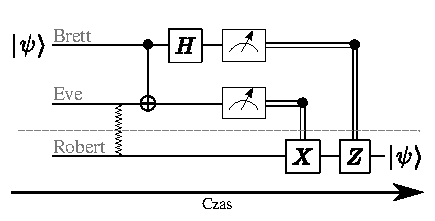
\includegraphics[width=0.8\textwidth]{pics/teleportation} \caption{Obwód
		teleportacji kwantowej. Linie poziome oznaczają kubity. Pionowa linia
		zygzakowata oznacza stan splątany. Linie podwójne oznaczają klasyczne bity.
		Pozioma linia przerywana oddziela układy Bretta i Alice od~układu Roberta.}
	\label{rys:teleportacja}
\end{figure}


Ponieważ nie~wiemy nic o~stanie kubitu Bretta, zapiszmy go w~ogólnej postaci
$$
	\ket{\psi} = \alpha \ket{0} + \beta \ket{1}.
$$
Wówczas stan początkowy układu jest następujący:
\begin{equation*}
	\begin{split}
		\ket{\psi_{t=0}} &=  \ket{\psi} \otimes \ket{\Phi^+}  =\\
		&= \ket{\psi} \otimes \frac{1}{\sqrt{2}}\left( \ket{0} \otimes \ket{0} +\ket{1} \otimes \ket{1} \right) = \\
		&= \left(\alpha \ket{0} + \beta  \ket{1}\right) \otimes \frac{1}{\sqrt{2}}\left( \ket{0} \otimes \ket{0} +\ket{1} \otimes \ket{1} \right)= \\
		&= \frac{1}{\sqrt{2}} \left(\alpha \ket{000} + \alpha \ket{011} + \beta  \ket{100} + \beta  \ket{111}  \right).
	\end{split}
\end{equation*}
Eve nakłada teraz bramkę~$\mat{CNOT}_1^2$ na~kubity swój i
Bretta\footnote{Jest to możliwe, jeśli zakładamy, że Eve może zbliżyć swój
	kubit do kubitu Bretta i~nakładać bramki jedno- i dwukubitowe na oba
	kubity.}, a~stan układu zmienia~się na~:
\begin{equation*}
	\begin{split}
		\ket{\psi_{t=1}} &= (\mat{CNOT}_1^2\otimes \mat{\id}) \frac{1}{\sqrt{2}} \left(\alpha \ket{000} + \alpha \ket{011} + \beta \ket{100} + \beta \ket{111}  \right) =\\
		&=\frac{1}{\sqrt{2}} \left(\alpha \ket{000} + \alpha \ket{011} + \beta \ket{110} + \beta \ket{101}  \right).
	\end{split}
\end{equation*}
Następnie Eve nakłada bramkę Hadamarda na~kubit Bretta, i~w~ten sposób zmienia stan na:
\begin{equation*}
	\begin{split}
		\ket{\psi_{t=2}} &=( \mat{H}\otimes\mat{\id}\otimes\mat{\id}) \frac{1}{\sqrt{2}} \left(\alpha \ket{000} + \alpha \ket{011} + \beta \ket{110} + \beta \ket{101}  \right) =\\
		&= \frac{1}{\sqrt{2}} \Big(
		\alpha \frac{1}{\sqrt{2}}(\ket{0}+\ket{1})\otimes (\ket{00} +  \ket{11}) + \\
		& + \beta \frac{1}{\sqrt{2}}(\ket{0}-\ket{1})\otimes(\ket{10} + \ket{01}) \Big) =\\
		&= \frac{1}{2} (\alpha \ket{000} + \alpha \ket{100}  + \alpha \ket{011} + \alpha \ket{111} + \\
		&+ \beta \ket{010} + \beta \ket{001} - \beta \ket{110} - \beta \ket{101} ).
	\end{split}
\end{equation*}
Następnie Eve mierzy pierwsze dwa kubity przy~użyciu pomiaru częściowego $\mathcal{P}$ składającego~się z~macierzy
\begin{equation*}
	\begin{split}
		\mathcal{P} = \{&\mat{P}_{00?}=\ketbra{0}{0}\otimes\ketbra{0}{0}\otimes\mat{\id}, \mat{P}_{01?}=\ketbra{0}{0}\otimes\ketbra{1}{1}\otimes\mat{\id}, \\
		&\mat{P}_{10?}=\ketbra{1}{1}\otimes\ketbra{0}{0}\otimes\mat{\id}, \mat{P}_{11?}=\ketbra{1}{1}\otimes\ketbra{1}{1}\otimes\mat{\id}\}
	\end{split}
\end{equation*}
i~otrzymuje -- w~zależności od~wyniku pomiaru -- z~jednakowym prawdopodobieństwem stany:
\begin{itemize}
	\item dla wyniku $00?$: $$\frac{1}{\sqrt{2}}\left(\alpha \ket{000}  + \beta \ket{001}\right) = \frac{1}{\sqrt{2}}\left(\ket{00}\otimes \ket{\psi}\right),$$
	\item dla wyniku $01?$: $$\frac{1}{\sqrt{2}}\left(\alpha \ket{011}  + \beta \ket{010}\right) = \frac{1}{\sqrt{2}}\left(\ket{01}\otimes \mat{Z}\ket{\psi}\right),$$
	\item dla wyniku $10?$: $$\frac{1}{\sqrt{2}}\left(\alpha \ket{100}  - \beta \ket{101}\right) = \frac{1}{\sqrt{2}}\left(\ket{10}\otimes \mat{X}\ket{\psi}\right),$$
	\item dla wyniku $11?$: $$\frac{1}{\sqrt{2}}\left(\alpha \ket{111}  - \beta \ket{110}\right) = \frac{1}{\sqrt{2}}\left(\ket{11}\otimes \mat{X}\mat{Z}\ket{\psi}\right).$$
\end{itemize}

Zauważmy, że~w~zależności od~wyniku pomiaru Eve stan kubitu Roberta jest
w tym momencie jednym z~czterech stanów: $\ket{\psi}$,
$\mat{Z}\ket{\psi}$, $\mat{X}\ket{\psi}$ lub~$\mat{X}\mat{Z}\ket{\psi}$.
Widać zatem, że~jeżeli~Robert wie, jaki wynik uzyskuje Eve, może~--
przy~użyciu kombinacji bramek $\mat{X}$ i~$\mat{Z}$ -- zmienić swój stan
tak, by~odzyskać oryginalny stan Bretta. W~przypadku wyniku pomiaru $00$
nie~musi robić nic; w~przypadku $01$ nakłada na~swój kubit bramkę
odwrotną do~$\mat{X}$, czyli~$\mat{X}^\dagger$; w~przypadku $10$ nakłada
bramkę $\mat{Z}^\dagger$, a~w~przypadku wyniku pomiaru $11$ -- bramki
$\mat{Z}^\dagger \mat{X}^\dagger$.

Zatem jeśli wykorzysta się splątanie kwantowe oraz~informację klasyczną, można
przenieść stan kubitu Bretta na~kubit Roberta, co może pozwolić
np.~na~kradzież kluczy do~zamków kwantowych, które opisywaliśmy
wcześniej. Na końcu tego rozdziału wyjaśnione jest jak doszło do kradzieży
klucza w komiksie.

% LTeX: language=pl-PL
\chapter{Podstawy matematyczne}\label{ch:podstawy}
\section{Liczby zespolone}
Czy~widział ktoś kiedyś liczbę? Na~przykład takie czterdzieści
dwa\footnote{Zobacz: Douglas Adams, ,,Autostopem przez~Galaktykę''.}? Czy można ją
zobaczyć? Możemy zobaczyć reprezentację liczby czterdzieści dwa w~postaci zapisu
dziesiętnego
\begin{quotation}
	\centering 42\index{forty two},
\end{quotation}
lub~binarnego
\begin{quotation}
	\centering 101010,
\end{quotation}
możemy też~zobaczyć czterdzieści dwa obiekty -- na~przykład ręczniki.
Jednak samej liczby zobaczyć nie~możemy, bo jest ona pojęciem abstrakcyjnym, które
istnieje niezależnie od~reprezentacji czy~interpretacji. Liczba czterdzieści dwa
jest liczbą naturalną. Tak samo jest z~liczbami wymiernymi i~rzeczywistymi ---
nie~możemy ich zobaczyć, dotknąć czy~powąchać; jednakże możemy na~nich działać.

Powyższe wprowadzenie ma Cię przekonać, że~liczby zespolone, o~których zaraz
będzie mowa, nie~są straszniejsze, dziwaczniejsze czy~bardziej abstrakcyjne
niż~liczby naturalne, całkowite, wymierne czy~rzeczywiste.
Dla~matematyka liczby są pewnymi obiektami, które mają pewną (mniej lub~bardziej elegancką)
strukturę matematyczną, między którymi istnieją relacje i~na~których można wykonywać pewne działania.
Dla~fizyka czy~inżyniera natomiast liczby służą do~opisu rzeczywistości:
naturalne -- do~zliczania obiektów, wymierne -- do~opisu stosunków między licznościami,
rzeczywiste -- do~mierzenia czasu, odległości, siły, a~zespolone -- do~opisywania prądu zmiennego,
fal lub~mechaniki kwantowej. Liczby zespolone stosowane są często tam, gdzie~mamy do~czynienia
z~obrotami lub~cyklicznie zmieniającymi~się wartościami.

Przejdźmy zatem do~rzeczy: zdefiniujmy liczby zespolone i~działania, jakie można
na~nich wykonywać.
Na~początek wprowadźmy jednostkę urojoną: ,,$\i$'', czyli~taką liczbę, dla której $\i^2=-1$.
Teraz możemy powiedzieć, że~\newterm{liczbą zespoloną}\index{liczba zespolona}
możemy nazwać dowolną liczbę $z$ taką, że
$$
	z = a + b \i,
$$
gdzie $a$ i~$b$ są liczbami rzeczywistymi. Samą liczbę $a$ nazywamy
\newterm{częścią
	rzeczywistą}\index{liczba zespolona!część rzeczywista} $z$ i~oznaczamy ją przez~$\Re z$,
a~$b$ nazywamy \newterm{częścią urojoną} \index{liczba zespolona!część urojona}
liczby $z$ i~oznaczamy przez~$\Im z$.
Zbiór liczb zespolonych oznacza~się przez~$\Complex$. Oznaczamy, że~$z$ należy do~zbioru~$\Complex$
-- albo~inaczej: że~jest liczbą zespoloną -- pisząc $z\in\Complex$.

Liczby zespolone przedstawia~się na~tzw.~płaszczyźnie zespolonej, na~której
na~osi poziomej odkłada~się wartość części rzeczywistej, a~na~osi pionowej -- wartość części urojonej.

\subsubsection{Moduł i~argument liczby zespolonej}
W~przypadku liczby zespolonej możemy mówić o~dwóch jej własnościach: module i~argumencie.
\newterm{Moduł liczby zespolonej}\index{liczba zespolona!moduł} zadany jest~-- jak
w~twierdzeniu Pitagorasa -- jako
$$
	\abs{z} = \abs{a+b\i} = \sqrt{a^2+b^2}.
$$
Należy zauważyć, że~moduł liczby zespolonej jest rzeczywisty i~zawsze większy lub~równy
zero. Moduł rozumiemy jako odległość liczby $z$ od~liczby $0=0+0\i$.

\newterm{Argumentem liczby zespolonej}\index{liczba zespolona!argument}
$z = a + bi \neq 0 + 0\i$ nazywamy liczbę rzeczywistą $\phi$ z~przedziału $[0,2\pi)$ spełniającą układ równań
$$
	\cos \phi = \frac{a}{\abs{z}}  \text{ oraz }   \sin \phi=\frac{b}{\abs{z}}.
$$
Inaczej można powiedzieć, że~argument liczby $z$ to wyrażona w~radianach wartość
kąta skierowanego $\phi$ pomiędzy osią rzeczywistą a~półprostą poprowadzoną od~środka układu
współrzędnych i~przechodzącą przez~punkt będący graficzną reprezentacją liczby $z$.
Ilustracją do~powyższych definicji jest Rysunek~\ref{rys:postaćgeometryczna}.

\subsubsection{Wzór Eulera}
Dla~liczby rzeczywistej $\phi$ możemy zapisać następującą relację, nazywaną wzorem Eulera\footnote{
	Leonhard Euler szwajcarski matematyk i fizyk (1707 -- 1783).}:
$$
	e^{\i \phi} = \cos\phi + \i \sin\phi.
$$
Zauważmy, że~dla~każdego $\phi\in \Real$ moduł liczby $|e^{\i \phi}| = 1$.

\subsubsection{Postać trygonometryczna liczby zespolonej}
Liczbę zespoloną $z = a + b\i \neq 0 + 0\i$ można zapisać w~postaci trygonometrycznej
$$
	z = \abs{z}(\cos \phi + \i \sin \phi),
$$
gdzie~$\phi$ jest argumentem liczby zespolonej.
Jeśli skorzystamy ze~wzoru Eulera, możemy zapisać liczbę $z$ jako
$$
	z = \abs{z}e^{\i \phi}.
$$
Warto dodać, że~w~fizyce moduł liczby nazywany jest często \newterm{amplitudą}\index{liczba zespolona!amplituda},
a~argument -- \newterm{fazą}\index{liczba zespolona!faza}.

\begin{figure}[h]
	\centering
	\resizebox{2in}{!}{
		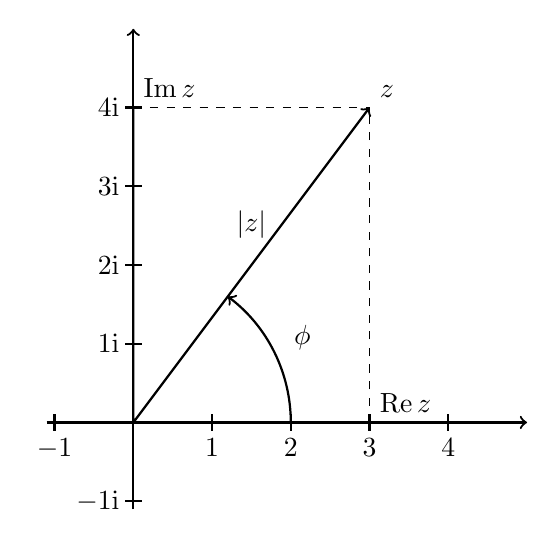
\begin{tikzpicture}
			\begin{scope}[thick,font=\normalsize]
				\draw
				(3,0) coordinate (a) node[above right] {$\Re z$}
				-- (0,0) coordinate (o)
				-- (0,4) coordinate (b) node[above right] {$\Im z$}
					[->] (0,0) -- (3,4) coordinate (z) node[above right] {$z$} node [above=6pt, midway]  {$\abs{z}$}
				pic["$\phi$", draw=black, ->, angle eccentricity=1.2, angle radius=2cm]
					{angle=a--o--z};
				\draw (3,0) -- (3,4) [dashed, thin];
				\draw (0,4) -- (3,4) [dashed, thin];

				\draw [->] (-1.1,0) -- (5,0) node [above left]  {};
				\draw [->] (0,-1.1) -- (0,5) node [below right] {};

				\foreach \n in {-1,...,-1,1,2,...,4}{%
						\draw (\n,-3pt) -- (\n,3pt)   node [below=5pt] {$\n$};
						\draw (-3pt,\n) -- (3pt,\n)   node [left=1ex] {$\n \i$};
					}
			\end{scope}
		\end{tikzpicture}
	}
	\caption{Płaszczyzna zespolona. Liczba zespolona $z=3+4\i$
		znajduje~się na~końcu strzałki. Moduł liczby $z$, oznaczony jako $|z|$,
		to długość strzałki. Wynosi on $\sqrt{3^2+4^2}=5$. Natomiast
		argument jest oznaczony jako $\phi$ i~wynosi $\arccos{\frac{3}{5}}\approx 0{,}92\ \mathrm{rad}.$}
	\label{rys:postaćgeometryczna}
\end{figure}

\subsubsection{Sprzężenie liczby zespolonej}
\newterm{Sprzężeniem liczby zespolonej}\index{liczba zespolona!sprzężenie} $z = a + b\i$ jest liczba
$$
	\conj{z} = a - b\i.
$$
Sprzężenie geometrycznie może być rozumiane jako odbicie symetryczne liczby wokół osi rzeczywistej.

\subsubsection{Operacje arytmetyczne na~liczbach zespolonych}
Dodawanie i~odejmowanie liczb zespolonych przeprowadza~się w~sposób naturalny, tzn.
jeśli~dodajemy dwie liczby zespolone $z_1 = a_1 + b_1 \i$ oraz~$z_2 = a_2 + b_2 \i$, to
ich suma wynosi
$
	z_1 + z_2 = (a_1 + a_2) + (b_1 + b_2) \i,
$
a~ich różnica
$
	z_1 - z_2 = (a_1 - a_2) + (b_1 - b_2) \i.
$
Geometryczna interpretacja dodawania
liczb zespolonych jest podana na~Rysunku~\ref{rys:dodawaniezespolonych}.

\begin{figure}[b]
	\centering
	\subbottom[Dodawanie liczb zespolonych $z_1 = 2 + 1\i$ oraz $z_2 = 1 + \frac{3}{2}\i$.\label{rys:dodawaniezespolonych}]%
	{
		\resizebox{0.46\textwidth}{!}{
			\centering
			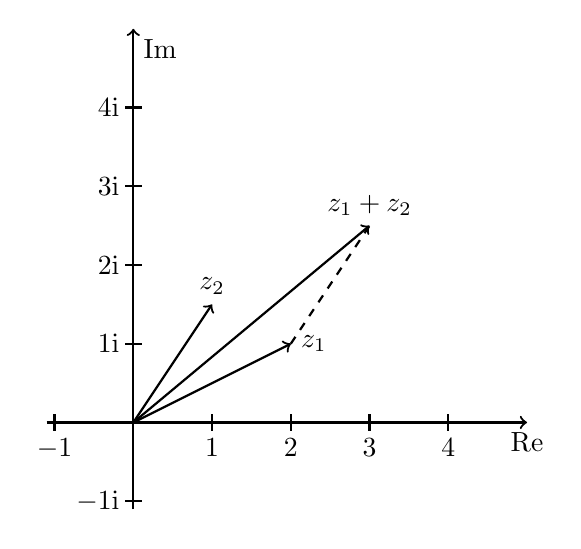
\begin{tikzpicture}
				\begin{scope}[thick,font=\normalsize]

					\draw [->] (-1.1,0) -- (5,0) node [below]  {$\Re$};
					\draw [->] (0,-1.1) -- (0,5) node [below right] {$\Im$};


					\draw [->] (0,0) -- (2,1) node [right]  {$z_1$};
					\draw [->] (0,0) -- (1,1.5) node [above]  {$z_2$};

					\draw  [dashed] (2,1) -- (3,2.5) ;
					\draw [->] (0,0) -- (3,2.5) node [above]  {$z_1+z_2$};

					\foreach \n in {-1,...,-1,1,2,...,4}{%
							\draw (\n,-3pt) -- (\n,3pt)   node [below=5pt] {$\n$};
							\draw (-3pt,\n) -- (3pt,\n)   node [left=1ex] {$\n \i$};
						}
				\end{scope}
			\end{tikzpicture}
		}
	}\hfill
	\subbottom[Mnożenie liczb zespolonych $z_1 = 3 + \frac{1}{2}\i$ oraz~$z_2 = 1 + 1\i$. Aby~uzyskać ich iloczyn, musimy pomnożyć amplitudy i~dodać fazy.\label{rys:mnożeniezespolonych}]%
	{
		\resizebox{0.46\textwidth}{!}{
			\centering
			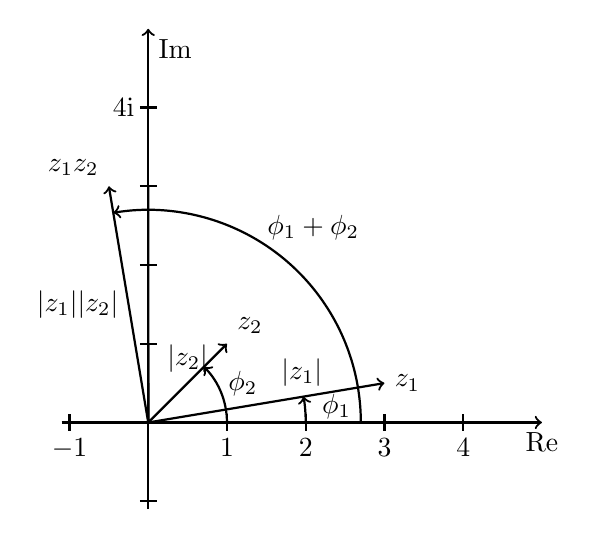
\begin{tikzpicture}
				\begin{scope}[thick,font=\normalsize]

					\draw
					(3,0) coordinate (a)
					-- (0,0) coordinate (o)
					-- (0,0.5) coordinate (b)
					[->] (0,0) -- (3	,0.5) coordinate (z) node[right] {$z_1$} node [above, pos=0.65]  {$\abs{z_1}$}
					pic["$\phi_1$", draw=black, ->, angle eccentricity=1.2, angle radius=2cm]
						{angle=a--o--z};

					\draw
					(1,0) coordinate (a)
					-- (0,0) coordinate (o)
					-- (0,1) coordinate (b)
					[->] (0,0) -- (1,1) coordinate (z) node[above right] {$z_2$} node [above=0.15, midway]  {$\abs{z_2}$}
					pic["$\phi_2$", draw=black, ->, angle eccentricity=1.3, angle radius=1cm]
						{angle=a--o--z};

					\draw
					(0.5,0) coordinate (a)
					-- (0,0) coordinate (o)
					-- (0,3) coordinate (b)
					[->] (0,0) -- (-0.5,3) coordinate (z) node[above left] {$z_1 z_2$} node [left, midway]  {$\abs{z_1}\abs{z_2}$}
					pic["$\phi_1 + \phi_2$", draw=black, ->, angle eccentricity=1.2, angle radius=2.7cm]
						{angle=a--o--z};

					\draw [->] (-1.1,0) -- (5,0) node [below]  {$\Re$};
					\draw [->] (0,-1.1) -- (0,5) node [below right] {$\Im$};

					\foreach \n in {-1,...,-1,1,2,...,4}{
							\draw (\n,-3pt) -- (\n,3pt)   node [below=5pt] {$\n$};
						}
					\foreach \n in {-1,...,-1,1,2,...,3}{
							\draw (-3pt,\n) -- (3pt,\n) ;
						}
					\foreach \n in {4}{
							\draw (-3pt,\n) -- (3pt,\n)   node [left=1ex] {$\n \i$};
						}

				\end{scope}
			\end{tikzpicture}
		}
	}
	\caption{Graficzna reprezentacja dodawania i~mnożenia liczb zespolonych}
	\label{rys:dodawanieimnożeniezespolonych}
\end{figure}

Mnożenie i~dzielenie liczb zespolonych jest nieco mniej intuicyjne. Jeśli~dane
są $z_1$ i~$z_2$ takie jak powyżej, ich iloczyn wynosi
\begin{equation*}
	\begin{split}
		z_1 z_2 =&(a_1+b_1 \i) (a_2 + b_2 \i)=
		\\=&a_1 a_2 + a_1 b_2 \i + b_1 a_2 i - b_1 b_2 = (a_1 a_2 - b_1 b_2) + (a_1 a_2 + b_1 b_2)\i,
	\end{split}
\end{equation*}
a~ich iloraz wynosi
$$ \frac{z_1}{z_2} =
	\frac{a_1 + b_1\i}{a_2 +b_2\i} =
	\frac{\left(a_1 + b_1\i\right) \cdot \left(a_2 - b_2\i\right)}
	{\left (a_2 + b_2\i\right) \cdot \left (a_2 - b_2\i\right)} =
	\left({a_1a_2 + b_1b_2 \over a_2^2 + b_2^2}\right) \left( {b_1a_2 - a_1b_2 \over a_2^2 + b_2^2} \right)\i.
$$

Mnożenie i~dzielenie liczb zespolonych łatwiej objaśnić z~wykorzystaniem postaci
trygonometrycznej. Jeżeli
$z_1 = \abs{z_1}e^{\i \phi_1}$, a $z_2 = \abs{z_2}e^{\i \phi_2}$, to
$$
	z_1 z_2 = \abs{z_1} \abs{z_2} e^{\i (\phi_1+\phi_2)}
	\text{ oraz } \frac{z_1}{z_2} = \frac{\abs{z_1}}{\abs{z_2}} e^{\i (\phi_1 - \phi_2)}.
$$
Geometryczna interpretacja mnożenia
liczb zespolonych jest podana na~Rysunku~\ref{rys:mnożeniezespolonych}.

Korzystając z powyższych faktów, policzmy wartość $\conj{z}z$
dla~liczby zespolonej $z=a+b\i$:
$$\conj{z}z = \conj{(a+b\i)}(a+b\i) =
	(a-b\i)(a+b\i) = a^2 - b^2\i^2 = a^2+b^2 = \abs{z}^2.$$
Wyrażenie to będzie nam później potrzebne.

\section{Wektory}
Niech~dany będzie pewien zbiór, którego elementy możemy do~siebie dodawać i~mnożyć~je
przez~liczby rzeczywiste lub~zespolone.
Dodatkowo załóżmy, że~operacje te zachowują~się zgodnie z~regułami wymienionymi
poniżej. Taki zbiór nazywamy \newterm{przestrzenią
	wektorową}\index{przestrzeń wektorowa}, a~elementy tego zbioru -- \newterm{wektorami}\index{wektor}.
Będziemy je tutaj oznaczać przez~$\ket{v}$, zamiast, jak to często bywa w~zwyczaju,
przez~$\vec{v}$. Oznaczenie $\ket{v}$ czytamy jako ,,\newterm{ket}\index{ket} v''.
Stosuje~się~je w~mechanice kwantowej,
a~pochodzi ono z~tzw.~notacji Diraca\footnote{Od~nazwiska angielskiego
	fizyka Paula Diraca (1902 -- 1984).}, którą posługujemy się w~tej książce.

Dla~nas wektory są kolekcją liczb. Gdy~te liczby są rzeczywiste, mówimy o~\emph{rzeczywistej przestrzeni wektorowej};
gdy~zespolone -- o~\emph{zespolonej przestrzeni wektorowej}.

Gdy~mówi~się o~wektorach, wiele osób odruchowo wyobraża je sobie jako strzałki
na~płaszczyźnie. My jednak posługujemy~się abstrakcyjnymi wektorami
w~przestrzeniach, które mają wiele wymiarów. Zatem dla~nas to wyobrażenie nie~będzie przydatne.
Jednakże~trzeba zaznaczyć, że~wszystkie własności wektorów wprowadzane w tym rozdziale odnoszą się również do~zwykłych wektorów na~płaszczyźnie.

Wymagamy, aby~wektory posiadały własności wymienione poniżej. Na początek
zaznaczmy, iż~spośród wektorów wyróżniamy jeden wektor $0$, który nazywamy
wektorem zerowym. Niech $\ket{u}, \ket{v}, \ket{z}$ oznaczają wektory,
a~$\alpha, \beta$ oznaczają liczby (skalary). Korzystając z~tych założeń,
prezentujemy listę wymaganych własności wektorów:
\begin{itemize}
	\item Przemienność dodawania:
	      $\ket{u}+\ket{v}=\ket{v}+\ket{u}$;

	\item Łączność dodawania wektorów:
	      $(\ket{u}+\ket{v})+\ket{z}=\ket{u}+(\ket{v}+\ket{z})$;

	\item Dla~każdego wektora $\ket{u}$ zachodzi
	      $0+\ket{u}=\ket{u}+0=\ket{u}$;

	\item Dla~każdego wektora $\ket{u}$ istnieje wektor przeciwny -$\ket{u}$ taki, że $$\ket{u}+(-\ket{u})=0;$$

	\item Łączność mnożenia przez~skalar:
	      $\alpha(\beta\ket{u})=(\alpha\beta)\ket{u};$

	\item Rozdzielność dodawania skalarów względem mnożenia przez~wektor:
	      $$(\alpha+\beta)\ket{u}=\alpha\ket{u}+\beta\ket{u};$$

	\item Rozdzielność dodawania wektorów względem~mnożenia przez~skalar:\\
	      $$\alpha(\ket{u}+\ket{v})=\alpha\ket{u}+\alpha\ket{v};$$

	\item 1 razy wektor daje ten sam wektor: $1\ket{u}=\ket{u}.$
\end{itemize}

\subsection{Wektory kolumnowe}
Zapiszmy pionową jednokolumnową tablicę $n$ liczb\index{wektor!kolumnowy}:
$$
	\begin{bmatrix}
		x_1    \\
		x_2    \\
		\vdots \\
		x_{n}  \\
	\end{bmatrix}.
$$
Działanie mnożenia takiej tablicy przez~skalar możemy wprowadzić $\alpha$ w~następujący sposób:
$$
	\alpha
	\begin{bmatrix}
		x_1    \\
		x_2    \\
		\vdots \\
		x_{n}  \\
	\end{bmatrix}=
	\begin{bmatrix}
		\alpha x_1   \\
		\alpha x_2   \\
		\vdots       \\
		\alpha x_{n} \\
	\end{bmatrix}.
$$
Możemy też~wprowadzić dodawanie takich tablic:
$$
	\begin{bmatrix}
		x_1    \\
		x_2    \\
		\vdots \\
		x_{n}  \\
	\end{bmatrix} +
	\begin{bmatrix}
		y_1    \\
		y_2    \\
		\vdots \\
		y_{n}  \\
	\end{bmatrix} =
	\begin{bmatrix}
		x_1 + y_1     \\
		x_2 + y_2     \\
		\vdots        \\
		x_{n} + y_{n} \\
	\end{bmatrix}.
$$
Zauważmy zatem, że~w~ten sposób możemy wprowadzić
konkretną reprezentację wektorów. Jeżeli~liczby: $\alpha$,
$x_1, x_2, \ldots, x_{n}$ oraz~$y_1, y_2, \ldots, y_{n}$ są rzeczywiste~-- to zbiór takich wektorów kolumnowych oznaczamy przez~$\Real^n$.
Jeżeli liczby~te są zespolone, to oznaczamy taki zbiór jako
$\Complex^n$.

\subsection{Wektory wierszowe}
Podobnie do~wektorów kolumnowych możemy zapisać wektory wierszowe\index{wektor!wierszowy}, np.~taki jak poniżej:
$$
	\begin{bmatrix}
		x_1    &
		x_2    &
		\cdots &
		x_{n}
	\end{bmatrix}.
$$
Możemy łatwo zauważyć, że~takie wektory można dodawać ze~sobą i~mnożyć przez~skalar.
Wektory takie oznaczamy symbolem $\bra{u}$, który czytamy ,,\newterm{bra}\index{bra}~u''.

\subsubsection{Transpozycja}
Możemy teraz wprowadzić operację \newterm{transpozycji}\index{wektor!transpozycja} wektorów. Oznaczamy ją
przez~$\square^T$. Zamienia ona wektory wierszowe na~kolumnowe i~kolumnowe na~wierszowe, tzn.:
$$
	\begin{bmatrix}
		x_1    \\
		x_2    \\
		\vdots \\
		x_{n}  \\
	\end{bmatrix}^T
	=
	\begin{bmatrix}
		x_1    &
		x_2    &
		\cdots &
		x_{n}
	\end{bmatrix}
$$
oraz
$$
	\begin{bmatrix}
		x_1    &
		x_2    &
		\cdots &
		x_{n}
	\end{bmatrix}^T
	=
	\begin{bmatrix}
		x_1    \\
		x_2    \\
		\vdots \\
		x_{n}  \\
	\end{bmatrix}.
$$

\subsubsection{Sprzężenie hermitowskie}
Dla~wektorów wierszowych i~kolumnowych zespolonych możemy wprowadzić specyficzną
operację \newterm{sprzężenia hermitowskiego}\index{wektor!sprzężenie hermitowskie}, oznaczaną znakiem sztyletu~$\square^\dagger$, taką że
$$
	\begin{bmatrix}
		x_1    \\
		x_2    \\
		\vdots \\
		x_{n}  \\
	\end{bmatrix}^\dagger
	=
	\begin{bmatrix}
		\conj{x_1} &
		\conj{x_2} &
		\cdots     &
		\conj{x_{n}}
	\end{bmatrix}
$$
oraz
$$
	\begin{bmatrix}
		x_1    &
		x_2    &
		\cdots &
		x_{n}
	\end{bmatrix}^\dagger
	=
	\begin{bmatrix}
		\conj{x_1}   \\
		\conj{x_2}   \\
		\vdots       \\
		\conj{x_{n}} \\
	\end{bmatrix}.
$$

Dla~naszych potrzeb w mechanice kwantowej utożsamiamy sprzężenie hermitowskie
,,keta'' z~odpowiednim wektorem ,,bra'' oraz~sprzężenie hermitowskie ,,bra'' z~,,ketem'':
$$
	\ket{u}^\dagger = \bra{u} \text{oraz} \bra{u}^\dagger = \ket{u}.
$$

\subsubsection{Iloczyn skalarny}
\newterm{Iloczynem skalarnym}\index{iloczyn!skalarny} wektorów nazywamy funkcję,
która dla~dwóch wektorów, $\ket{u}$ i~$\ket{v}$, zwraca liczbę rzeczywistą lub~zespoloną,
która spełnia poniższe własności:

\begin{itemize}
	\item $\braket{u}{v}=\conj{\braket{v}{u}}$,
	\item  $(\alpha\bra{u})\ket{v} = \alpha\braket{u}{v}$,
	      $(\bra{u}+\bra{v})\ket{z}=\braket{u}{z}+\braket{v}{z}$,
	\item $\braket{u}{u}\geq 0$,
	\item $\braket{u}{u} = 0$ wtedy i~tylko wtedy, gdy~$\ket{u}=0$.
\end{itemize}

Przeprowadźmy teraz na~wektorach następującą operację:
niech~będą dane dwa wektory $\ket{u}, \ket{v}\in \Complex^n$, takie że
$$
	\ket{u} =
	\begin{bmatrix}
		x_1    \\
		x_2    \\
		\vdots \\
		x_{n}  \\
	\end{bmatrix},\quad
	\ket{v} =
	\begin{bmatrix}
		y_1    \\
		y_2    \\
		\vdots \\
		y_{n}  \\
	\end{bmatrix};\quad
$$
wówczas
$$
	\braket{u}{v} = \conj{x}_1 y_1 + \conj{x}_2 y_2 + \ldots + \conj{x}_n y_n
$$
nazywamy iloczynem skalarnym wektorów $\ket{u}$ oraz~$\ket{v}$\footnote{Matematycznie
	można zdefiniować inne iloczyny skalarne,
	ale~nam nie~będą one tu potrzebne.}. Skalarnie można mnożyć tylko wektory o~tej
samej liczbie elementów. Wynikiem iloczynu skalarnego jest liczba.

\subsection{Kombinacja liniowa wektorów}
Gdy~mamy dane dwie liczby, $\alpha$ i~$\beta$, oraz~dwa wektory, $\ket{u}$ i~$\ket{v}$,
możemy uzyskać taki wektor
$$
	\ket{z} = \alpha \ket{u} + \beta \ket{v},
$$
który nazywamy \newterm{kombinacją liniową wektorów}\index{kombinacja liniowa
	wektorów}
$\ket{u}$ i~$\ket{v}$ o~współczynnikach $\alpha$ i~$\beta$.
A~ogólniej: wektor
$$
	\ket{z} = \alpha_1 \ket{u_1} + \alpha_2 \ket{u_2} + \ldots + \alpha_n \ket{u_n}
$$
nazywamy kombinacją liniową wektorów $\ket{u_1}, \ket{u_2}, \ldots, \ket{u_n}$
o~współczynnikach $\alpha_1, \alpha_2, \ldots, \alpha_n$.

\subsection{Liniowa zależność wektorów}
Mając dany zbiór wektorów $\{\ket{u_1}, \ket{u_2}, \ldots, \ket{u_n}\}$, mówimy,
że~jest on \newterm{liniowo zależny}\index{liniowa zależność wektorów}, jeżeli~istnieje
jeden taki wektor $\ket{u_i}$ oraz~niezerowe współczynniki $\alpha_1,
	\alpha_2, \ldots, \alpha_n$, takie że:
$$
	\alpha_i \ket{u_i} = \alpha_1 \ket{u_1} + \alpha_2 \ket{u_2} +
	\ldots + \alpha_{i-1} \ket{u_{i-1}} + \alpha_{i+1} \ket{u_{i+1}} + \ldots + \alpha_n \ket{u_n}.
$$
Oznacza to, że~jeden z~wektorów można zapisać jako kombinację liniową pozostałych wektorów, której współczynniki są niezerowe.

\subsection{Baza i~wymiar przestrzeni wektorowej}
Jeżeli~zbiór $n$ wektorów $\{\ket{u_1}, \ket{u_2}, \ldots, \ket{u_n}\}$
należących do~danej przestrzeni wektorowej nie~jest
liniowo zależny i~dodanie dowolnego wektora niezerowego z~tej przestrzeni
do~zbioru spowoduje, że~stanie~się on liniowo zależny, to taki zbiór nazywamy \newterm{bazą przestrzeni
	wektorowej}\index{baza!przestrzeni wektorowej}. Wówczas~mówimy, że~przestrzeń
wektorowa ma \newterm{wymiar}\index{przestrzeń wektorowa!wymiar} $n$.
Każda przestrzeń wektorowa ma bazę.

Dowolny wektor możemy zapisać jako kombinację wektorów bazowych.
Nas natomiast interesują tylko bazy, które jednocześnie tworzą zbiór
ortonormalny, tzn.~taki, że~dla~wektorów z~bazy $\{\ket{e_1}, \ket{e_2}, \ldots
	\ket{e_n}\}$ zachodzi $\braket{e_i}{e_j}=0$ dla~$i\neq j$ dla~$i=1,2,\ldots,n$ i~$j=1,2,\ldots,n$ oraz~$\braket{e_i}{e_i}=0$
dla~$i=1,2,\ldots,n$. Wtedy wektor
$\ket{u}$ zapisujemy w~następujący sposób:
$$
	\ket{u}=\braket{e_1}{u}\ket{e_1} + \braket{e_2}{u}\ket{e_2} + \ldots + \braket{e_n}{u}\ket{e_n}.
$$

W~przypadku wektorów kolumnowych jedną bazę wyróżnia~się szczególnie i~nazywa~się
ją \newterm{bazą obliczeniową}\index{baza!obliczeniowa}. Składa~się ona
z~wektorów:
$$
	\ket{0}=
	\begin{bmatrix}
		1      \\
		0      \\
		\vdots \\
		0      \\
	\end{bmatrix},
	\ket{1}=
	\begin{bmatrix}
		0      \\
		1      \\
		\vdots \\
		0      \\
	\end{bmatrix},
	\ket{n-1}=
	\begin{bmatrix}
		0      \\
		0      \\
		\vdots \\
		1      \\
	\end{bmatrix}.
$$
Zapamiętajmy: nie~należy mylić wektora zerowego $0$ z~wektorem $\ket{0}$; ten pierwszy
składa~się z~samych zer, a~drugi ma na~pierwszej pozycji $1$.

\subsection{Norma euklidesowa}
Jeżeli~mamy zdefiniowany iloczyn skalarny wektorów, to możemy wprowadzić pojęcie
długości wektora -- lub~inaczej: \newterm{normy wektora}\index{wektor!norma}.
Normy wektorów powinny mieć następujące własności:
\begin{itemize}
	\item Dla~każdego wektora $\ket{u}$ i~liczby $\alpha$: $\norm{\alpha\ket{u}}=|a|\norm{\ket{u}}$;
	\item Dla~każdych dwóch wektorów $\ket{u}$ oraz~$\ket{v}$: $\norm{\ket{u}+\ket{v}}\leq \norm{\ket{u}}+\norm{\ket{v}}$;
	\item Tylko~i~wyłącznie dla~wektora zerowego $0$: $\norm{0}=0$.
\end{itemize}
Warto tu zauważyć, że~dla~każdego wektora $\ket{u}$ jego norma jest nieujemna
$\norm{\ket{u}}\geq 0$.
Nas będzie interesować tylko~i~wyłącznie \newterm{norma
	euklidesowa}\index{wektor!norma euklidesowa} wektora
$\norm{\ket{u}}=\sqrt{\braket{u}{u}}$.

W~przypadku wektora kolumnowego
$$
	\ket{u}=
	\begin{bmatrix}
		x_1    \\
		x_2    \\
		\vdots \\
		x_{n}  \\
	\end{bmatrix}
$$
mamy następujący wzór na~normę euklidesową:
\begin{equation*}
	\begin{split}
		\norm{\ket{u}}=\sqrt{\braket{u}{u}}
		& = \sqrt{\conj{x_1}x_1 + \conj{x_2}x_2 + \ldots + \conj{x_n}x_n}  \\
		&= \sqrt{\abs{x_1}^2 + \abs{x_2}^2 + \ldots + \abs{x_n}^2}.
	\end{split}
\end{equation*}
\subsection{Wektor unormowany}
Wektor $\ket{u}$, którego norma jest równa jeden $\norm{\ket{u}}=1$, nazywamy
\newterm{unormowanym}\index{wektor!unormowany}.

\subsection{Ortogonalność}
Dwa wektory $\ket{u}$ i~$\ket{v}$ nazywamy
\newterm{ortogonalnymi}\index{wektory!ortogonalne} (lub~inaczej --
prostopadłymi), gdy~ich iloczyn skalarny wynosi zero $\braket{u}{v}=0$. Jeżeli
wektory $\ket{u}$ i~$\ket{v}$ są unormowane i~ortogonalne, to nazywamy je
\newterm{ortonormalnymi}\index{wektory!ortonormalne}.

\section{Macierze}
\newterm{Macierzą}\index{macierz} nazywamy prostokątną tablicę liczb. Dla~nas
będą to liczby rzeczywiste lub~zespolone.
Przykładowo poniżej dana jest macierz o~wymiarach $m$ na~$n$:
$$
	\mat{A} =
	\begin{bmatrix}
		a_{11} & a_{12} & \cdots & a_{1n} \\
		a_{21} & a_{22} & \cdots & a_{2n} \\
		\vdots & \vdots & \ddots & \vdots \\
		a_{m1} & a_{m2} & \cdots & a_{mn}
	\end{bmatrix}.
$$

Liczby $a_{ij}$ nazywamy \newterm{elementami macierzowymi}\index{element macierzowy} albo~po~prostu
elementami macierzy.
Jeżeli~liczby $a_{ij}$ są rzeczywiste, to opisujemy macierz jako $\mat{A}\in
	\Real^{mn}$, natomiast jeżeli~są zespolone, opisujemy ją jako $\mat{A}\in\Complex^{mn}$. Dlatego
też~zamiast pisać za~każdym razem, że~mówimy o~macierzach lub~wektorach
rzeczywistych lub~zespolonych, będziemy stosować znak $\Field$\footnote{Z angielskiego \emph{field},
	czyli~ciało liczbowe.} jako zamiennik dla~$\Real$ oraz~$\Complex$.


\subsubsection{Dodawanie}
Jeżeli~mamy dwie macierze $\mat{A}, \mat{B}\in \Field^{mn}$ o~identycznych
rozmiarach, to możemy je dodawać do siebie, otrzymując macierz $\mat{A} +
	\mat{B}\in \Field^{mn}$. Zatem, jeśli dane są dwie poniższe macierze:
$$
	\mat{A} =
	\begin{bmatrix}
		a_{11} & a_{12} & \cdots & a_{1n} \\
		a_{21} & a_{22} & \cdots & a_{2n} \\
		\vdots & \vdots & \ddots & \vdots \\
		a_{m1} & a_{m2} & \cdots & a_{mn}
	\end{bmatrix}, \quad
	\mat{B} =
	\begin{bmatrix}
		b_{11} & b_{12} & \cdots & b_{1n} \\
		b_{21} & b_{22} & \cdots & b_{2n} \\
		\vdots & \vdots & \ddots & \vdots \\
		b_{m1} & b_{m2} & \cdots & b_{mn}
	\end{bmatrix},
$$
dodajmy je do siebie w~następujący sposób -- element po~elemencie:
$$
	\mat{A} + \mat{B} =
	\begin{bmatrix}
		a_{11} + b_{11} & a_{12} + b_{12} & \cdots & a_{1n} + b_{1n} \\
		a_{21} + b_{21} & a_{22} + b_{22} & \cdots & a_{2n} + b_{2n} \\
		\vdots          & \vdots          & \ddots & \vdots          \\
		a_{m1} + b_{m1} & a_{m2} + b_{m2} & \cdots & a_{mn} + b_{mn} \\
	\end{bmatrix}.
$$

\subsubsection{Mnożenie przez~skalar}
Mnożenie macierzy $\mat{A} \in \Field^{mn}$ przez~skalar $\alpha$ polega
na~pomnożeniu każdego elementu tej macierzy przez~dany skalar. W~wyniku tego
działania otrzymujemy macierz $\alpha\mat{A} \in \Field^{mn}$ o postaci
$$
	\alpha \mat{A} =
	\begin{bmatrix}
		\alpha a_{11} & \alpha a_{12} & \cdots & \alpha a_{1n} \\
		\alpha a_{21} & \alpha a_{22} & \cdots & \alpha a_{2n} \\
		\vdots        & \vdots        & \ddots & \vdots        \\
		\alpha a_{m1} & \alpha a_{m2} & \cdots & \alpha a_{mn}
	\end{bmatrix}.
$$

\subsubsection{Transpozycja}
\newterm{Transpozycja macierzy}\index{macierz!transpozycja} $\mat{A} \in
	\Field^{mn}$ polega na~zamianie wierszy tej
macierzy z~jej kolumnami. Otrzymujemy wówczas macierz $\mat{A}^T \in
	\Field^{nm}$ o postaci
$$\mat{A}^T =
	\begin{bmatrix}
		a_{11} & a_{21} & \cdots & a_{m1} \\
		a_{12} & a_{22} & \cdots & a_{m2} \\
		\vdots & \vdots & \ddots & \vdots \\
		a_{1n} & a_{2n} & \cdots & a_{mn}
	\end{bmatrix}.
$$


\subsubsection{Sprzężenie hermitowskie}
\newterm{Sprzężenie hermitowskie macierzy}\index{macierz!sprzężenie
	hermitowskie} $\mat{A} \in \Field^{mn}$ to połączenie
transpozycji macierzy ze~sprzężeniem zespolonym każdego jej elementu; zatem
$\mat{A}^\dagger \in \Field^{nm}$ ma postać
$$
	\mat{A}^\dagger =
	\begin{bmatrix}
		\conj{a_{11}} & \conj{a_{21}} & \cdots & \conj{a_{m1}} \\
		\conj{a_{12}} & \conj{a_{22}} & \cdots & \conj{a_{m2}} \\
		\vdots        & \vdots        & \ddots & \vdots        \\
		\conj{a_{1n}} & \conj{a_{2n}} & \cdots & \conj{a_{mn}}
	\end{bmatrix}.
$$
Zauważmy, że~dla macierzy rzeczywistych sprzężenie hermitowskie i~transpozycja zachowują~się tak samo.

\subsubsection{Mnożenie macierzy przez~wektor kolumnowy}
Mnożenie macierzy $\mat{A}\in \Field^{mn}$ z~prawej strony przez~wektor
kolumnowy $\ket{x}\in \Field^{n}$ polega na~policzeniu sumy iloczynów elementów
macierzy z~odpowiednimi elementami wektora. Otrzymujemy wtedy $\mat{A}\ket{x}\in
	\Field^m$:
$$
	\mat{A} =
	\begin{bmatrix}
		a_{11} & a_{12} & \cdots & a_{1n} \\
		a_{21} & a_{22} & \cdots & a_{2n} \\
		\vdots & \vdots & \ddots & \vdots \\
		a_{m1} & a_{m2} & \cdots & a_{mn}
	\end{bmatrix}, \quad
	\ket{x}=
	\begin{bmatrix}
		x_1    \\
		x_2    \\
		\vdots \\
		x_{n}  \\
	\end{bmatrix},
$$

$$
	\mat{A} \ket{x}=
	\begin{bmatrix}
		a_{11}x_1 + a_{12}x_2 + \dots + a_{1n}x_n \\
		a_{21}x_1 + a_{22}x_2 + \dots + a_{2n}x_n \\
		\vdots                                    \\
		a_{m1}x_1 + a_{m2}x_2 + \cdots + a_{mn}x_n
	\end{bmatrix}.
$$
Zauważmy, że~liczba elementów wektora ,,wejściowego'' odpowiada liczbie wierszy
macierzy, a~liczba elementów wektora ,,wyjściowego'' odpowiada liczbie kolumn.

\subsubsection{Mnożenie macierzy przez~macierz}
Operacje dodawania i~mnożenia macierzy przez~skalar są intuicyjne.
\newterm{Mnożenie macierzy}\index{iloczyn!macierzowy} przez siebie
jest nieco bardziej złożone. Jeżeli mamy dane macierze $\mat{A}\in\Field^{mk}$ oraz
$\mat{B}\in\Field^{kn}$ o postaciach
$$
	\mat{A} =
	\begin{bmatrix}
		a_{11} & a_{12} & \cdots & a_{1k} \\
		a_{21} & a_{22} & \cdots & a_{2k} \\
		\vdots & \vdots & \ddots & \vdots \\
		a_{m1} & a_{m2} & \cdots & a_{mk}
	\end{bmatrix}, \quad
	\mat{B} =
	\begin{bmatrix}
		b_{11} & b_{12} & \cdots & b_{1n} \\
		b_{21} & b_{22} & \cdots & b_{2n} \\
		\vdots & \vdots & \ddots & \vdots \\
		b_{k1} & b_{k2} & \cdots & b_{kn}
	\end{bmatrix},
$$
to wynikiem ich wymnożenia jest macierz $\mat{C}\in\Field^{mn}$
$$
	\mat{C} =
	\begin{bmatrix}
		c_{11} & c_{12} & \cdots & c_{1n} \\
		c_{21} & c_{22} & \cdots & c_{2n} \\
		\vdots & \vdots & \ddots & \vdots \\
		c_{m1} & c_{m2} & \cdots & c_{mn}
	\end{bmatrix},
$$
taka że~jej elementy macierzowe $c_{ij}$ mają następującą postać:
$$c_{ij}=a_{i1}b_{1j} + a_{i2}b_{2j} + \dots + a_{ik}b_{kj} \text{ dla } i=1,2,\dots, m \text{ oraz } j=1,2,\dots, n.$$

Iloczyn macierzowy można rozumieć również w~następujący sposób: jeżeli~zapiszemy
macierz $\mat{A}$ jako wektor kolumnowy wektorów wierszowych
$$
	\mat{A} = \begin{bmatrix}
		\bra{a_1} \\
		\bra{a_2} \\
		\vdots    \\
		\bra{a_k}
	\end{bmatrix},
$$
gdzie $\bra{a_1} = \begin{bmatrix}a_{11} & a_{12} & \dots & a_{1k} \end{bmatrix},
	\bra{a_2} = \begin{bmatrix}a_{21} & a_{22} & \dots & a_{2k} \end{bmatrix}, \dots,
	\bra{a_m} = \begin{bmatrix}a_{m1} & a_{m2} & \dots & a_{mk} \end{bmatrix}$,
natomiast macierz $\mat{B}$ jako wektor wierszowy wektorów kolumnowych
$$
	\mat{B} = \begin{bmatrix}
		\ket{b_1} &
		\ket{b_2} &
		\dots     &
		\ket{b_n}
	\end{bmatrix},
$$
gdzie
$$
	\ket{b_1} =
	\begin{bmatrix}
		b_{11} \\
		b_{21} \\
		\vdots \\
		b_{k1}
	\end{bmatrix}, \quad
	\ket{b_1} =
	\begin{bmatrix}
		b_{12} \\
		b_{22} \\
		\vdots \\
		b_{k2}\end{bmatrix},\quad \dots, \quad
	\ket{b_1} =
	\begin{bmatrix}
		b_{1n} \\
		b_{2n} \\
		\vdots \\
		b_{kn}
	\end{bmatrix},
$$
to iloczyn macierzy $\mat{C}=\mat{A}\mat{B}$ można zapisać jako macierz iloczynów skalarnych
$$
	\mat{C}=
	\begin{bmatrix}
		\braket{a_1}{b_1} & \braket{a_1}{b_2} & \cdots & \braket{a_1}{b_n} \\
		\braket{a_2}{b_1} & \braket{a_2}{b_2} & \cdots & \braket{a_2}{b_n} \\
		\vdots            & \vdots            & \ddots & \vdots            \\
		\braket{a_m}{b_1} & \braket{a_m}{b_2} & \cdots & \braket{a_m}{b_n} \\
	\end{bmatrix}.
$$
\subsubsection{Macierz zerowa}
Macierz $\mat{0}\in \Field^{mn}$, która składa~się z~samych zer
$$
	\mat{0}=
	\begin{bmatrix}
		0      & 0      & \cdots & 0      \\
		0      & 0      & \cdots & 0      \\
		\vdots & \vdots & \ddots & \vdots \\
		0      & 0      & \cdots & 0      \\
	\end{bmatrix},
$$
nazywamy \newterm{zerową}\index{macierz!zerowa}.
Dla~dowolnych macierzy $\mat{A}\in \Field^{km}$ oraz~$\mat{B}\in \Field^{nl}$
mamy
$$
	\mat{A}\mat{0} = \mat{0}\in \Field^{kn}, \ \mat{0}\mat{B} = \mat{0}\in \Field^{ml}.
$$

\subsubsection{Macierz diagonalna}
Macierz kwadratowa $\mat{A}_m\in \Field^{mm}$, która wygląda następująco:
$$
	\mat{A} =
	\begin{bmatrix}
		a_{11} & 0      & \cdots & 0      \\
		0      & a_{22} & \cdots & 0      \\
		\vdots & \vdots & \ddots & \vdots \\
		0      & 0      & \cdots & a_{mm}
	\end{bmatrix},
$$
nazywana jest \newterm{macierzą diagonalną}\index{macierz!diagonalna}.
Elementy $a_{11}, a_{22}, \ldots, a_{mm}$ nazywane są \newterm{przekątną
	macierzy}\index{przekątna macierzy} bądź~jej
\newterm{diagonalą}\index{diagonala}.

\subsubsection{Macierz jednostkowa}
Macierz kwadratową $\mat{\id}_m\in \Field^{mm}$ diagonalną, która ma jedynki na~przekątnej
$$
	\mat{\id}_m=
	\begin{bmatrix}
		1      & 0      & \cdots & 0      \\
		0      & 1      & \cdots & 0      \\
		\vdots & \vdots & \ddots & \vdots \\
		0      & 0      & \cdots & 1      \\
	\end{bmatrix},
$$
nazywamy \newterm{jednostkową}\index{macierz!jednostkowa}. Macierz taka zachowuje~się
w~mnożeniu macierzowym jak~$1$ w~mnożeniu skalarnym. Weźmy macierze
$\mat{A}\in \Field^{km}$ oraz
$\mat{B}\in \Field^{mn}$. Uzyskamy wtedy
$$
	\mat{A}\mat{\id}_m = \mat{A}, \ \mat{\id}_m\mat{B} = \mat{B}.
$$

\subsubsection{Macierz odwrotna}
Dla~macierzy kwadratowej $\mat{A}\in \Field^{mm}$ może (ale~nie~musi) istnieć macierz $\mat{A}^{-1}\in \Field^{mm}$, która daje
$$
	\mat{A}\mat{A}^{-1} = \mat{A}^{-1}\mat{A} = \mat{\id}_m.
$$
Macierz $\mat{A}^{-1}$ nazywamy \newterm{odwrotną}\index{macierz!odwrotna} do~macierzy $\mat{A}$.
W~zależności od~tego, jaką jest macierz $\mat{A}$,
macierz $\mat{A}^{-1}$ może istnieć lub~nie. Nie~będziemy~się tu zajmować
warunkami istnienia macierzy odwrotnej, gdyż~-- jak zobaczymy później --
dla~macierzy nas interesujących macierze odwrotne będą istnieć zawsze i~w~dodatku
będą miały szczególną postać.

\subsubsection{Iloczyn Kroneckera}
Dla~danych dwóch macierzy $\mat{A}\in\Field^{mn}$ i~$\mat{B}\in\Field^{kl}$
wynikiem ich \newterm{iloczynu
	Kroneckera}\index{iloczyn!Kroneckera} jest taka macierz
$\mat{C}\in\Field^{m\times k, n\times l}$, która
powstaje przez~pomnożenie każdego elementu macierzowego macierzy $\mat{A}$
przez~całą macierz $\mat{B}$, tak jak w~poniższym wzorze:
$$
	\mat{C}=\mat{A}\otimes \mat{B}=
	\begin{bmatrix}
		a_{11}\mat{B} & a_{12}\mat{B} & \cdots & a_{1n}\mat{B} \\
		a_{21}\mat{B} & a_{22}\mat{B} & \cdots & a_{2n}\mat{B} \\
		\vdots        & \vdots        & \ddots & \vdots        \\
		a_{m1}\mat{B} & a_{m2}\mat{B} & \cdots & a_{mn}\mat{B} \\
	\end{bmatrix}.
$$
Zauważmy, że~wymiary macierzy wynikowej to $m\times k$ na~$n\times l$. Poniżej
wymienimy listę własności iloczynu Kroneckera, które są potrzebne
do~zrozumienia własności obwodów kwantowych:

\begin{itemize}
	\item Iloczyn Kroneckera nie~musi być przemienny: $\mat{A}\otimes \mat{B}\neq \mat{B} \otimes \mat{A};$
	\item Rozdzielność iloczynu Kroneckera względem dodawania:
	      $$
		      \mat{A} \otimes (\mat{B}+\mat{C}) = \mat{A} \otimes \mat{B} + \mat{A} \otimes \mat{C},
	      $$
	      $$
		      (\mat{A}+\mat{B})\otimes \mat{C} = \mat{A} \otimes \mat{C} + \mat{B} \otimes \mat{C};
	      $$
	\item Łączność mnożenia przez skalar:
	      $
		      (c\mat{A}) \otimes \mat{B} = \mat{A} \otimes (c\mat{B}) = c(\mat{A} \otimes \mat{B});
	      $
	\item Łączność iloczynu Kroneckera:
	      $
		      (\mat{A} \otimes \mat{B}) \otimes \mat{C} = \mat{A} \otimes (\mat{B} \otimes \mat{C});
	      $
	\item Jeżeli możemy pomnożyć macierze $\mat{A}$ i $\mat{C}$ oraz $\mat{B}$ i $\mat{D}$, to:
	      $$
		      (\mat{A} \otimes \mat{B})(\mat{C} \otimes \mat{D}) = (\mat{AC}) \otimes (\mat{BD});
	      $$
	\item Odwrotność:
	      $
		      (\mat{A} \otimes \mat{B})^{-1} = \mat{A}^{-1} \otimes \mat{B}^{-1};
	      $
	\item Transpozycja oraz~sprzężenie hermitowskie:
	      $$
		      (\mat{A}\otimes \mat{B})^\mathrm{T} = \mat{A}^\mathrm{T} \otimes \mat{B}^\mathrm{T}, \quad
		      (\mat{A}\otimes \mat{B})^\dagger = \mat{A}^\dagger \otimes \mat{B}^\dagger.
	      $$
\end{itemize}

\subsubsection{Iloczyn zewnętrzny}
Nazwą \newterm{iloczyn zewnętrzny}\index{iloczyn!zewnętrzny} wektora kolumnowego
$$
	\ket{u}=
	\begin{bmatrix}
		x_1    \\
		x_2    \\
		\vdots \\
		x_{n}  \\
	\end{bmatrix}
$$ i~wektora wierszowego
$$
	\bra{v}=
	\begin{bmatrix}
		y_1    &
		y_2    &
		\cdots &
		y_{m}
	\end{bmatrix}
$$
określamy macierz powstałą z iloczynu macierzowego tych wektorów:
$$
	\ketbra{u}{v}
	=\begin{bmatrix}
		x_1 y_1 & x_1 y_2 & \cdots & x_1 y_m \\
		x_2 y_1 & x_2 y_2 & \cdots & x_2 y_m \\
		\vdots  & \vdots  & \ddots & \cdots  \\
		x_n y_1 & x_n y_2 & \cdots & x_n y_m
	\end{bmatrix}.
$$

\subsubsection{Notacja Diraca}
W~tym miejscu mamy dość wiedzy, by docenić notację Diraca. Iloczyn skalarny
$\braket{u}{v}$ wektorów $\ket{u}$ i~$\ket{v}$ czytamy jako
,,\newterm{braket}\index{braket}~u~v''\footnote{Ang.,,bracket" -- nawias.}.
Natomiast iloczyn $\ketbra{u}{v}$ czytamy jako
,,\newterm{ketbra}\index{ketbra}~u~v''. Interesujące jest zatem wyrażenie
$\ket{u}\!\braket{v}{x}$, w~którym nawiasy możemy rozłożyć w~taki sposób:
$\ket{u}(\braket{v}{x})$ lub~tak: $(\ketbra{u}{v})\ket{x}$. Wzory te mają różne
znaczenie, ale~ponieważ sprowadzają~się one do~mnożenia macierzy, mają tę samą
wartość. Co ciekawe, od~razu można zauważyć, że~wyrażenie
$\ket{u}\!\braket{v}{x}$ jest równe wyrażeniu $\braket{v}{x}\ket{u}$, ponieważ
mnożenie skalara przez~wektor jest przemienne.


\subsection{Macierze unitarne}
Macierze kwadratowe, które przy~mnożeniu z~prawej strony przez~wektor
nie~zmieniają jego normy, nazywamy macierzami
\newterm{unitarnymi}\index{macierz!unitarna}.
Znaczy to, że~dla~każdego $\ket{u}\in \Field^{n}$ i~dla~każdej macierzy
unitarnej $\mat{U}\in \Field^{nn}$ mamy
$$
	\norm{\mat{U}\ket{u}}=\norm{\ket{u}}.
$$

Dla~każdej macierzy unitarnej $\mat{U}$ istnieje macierz odwrotna $\mat{U}^{-1}$, tzn.
$$
	\mat{U}\mat{U}^{-1} = \mat{U}^{-1}\mat{U} = \mat{\id}_m.
$$
Dlatego macierze unitarne często utożsamiane są z~obrotami.
Macierze unitarne mają pewną ciekawą własność -- ich odwrotność jest ich
sprzężeniem hermitowskim, tzn.~$\mat{U}^{-1} = \mat{U}^\dagger$.

Zauważmy, że~jeżeli macierz $\mat{U}$ przekształca $\ket{u}$ na~$\ket{v}$, to
macierz $\mat{U}^\dagger$ przekształca $\ket{v}$ na~$\ket{u}$, tzn.~jeżeli
$\ket{v} = \mat{U}\ket{u}$, to $\ket{u} = \mat{U}^\dagger\ket{v}.$

\subsection{Macierz hermitowska}
Macierz kwadratową, dla której jej sprzężenie hermitowskie jest równe samej macierzy, tj.
$$
	\mat{A} = \mat{A}^\dagger
$$
nazywamy \newterm{macierzą hermitowską}\footnote{Od nazwiska francuskiego matematyka Charles'a Hermite'a (1822 -- 1901).}\index{macierz!hermitowska}.

\section{Podsumowanie}
Przedstawiony powyżej formalizm matematyczny pozwala zrozumieć podstawy
informatyki kwantowej.
Zauważcie, że~zaczęliśmy ten dodatek od~liczb zespolonych -- czyli~pewnego opisu
obrotów na~płaszczyźnie -- a~skończyliśmy na~macierzach unitarnych, które opisują
obroty w~przestrzeniach wektorowych.


\end{document}
